%%%%%%%%%%%%%%%%%%%%%%%%%%%%%%%%%%%%%%%%%
% University Assignment Title Page 
% LaTeX Template
% Version 1.0 (27/12/12)
%
% This template has been downloaded from:
% http://www.LaTeXTemplates.com
%
% Original author:
% WikiBooks (http://en.wikibooks.org/wiki/LaTeX/Title_Creation)
%
% License:
% CC BY-NC-SA 3.0 (http://creativecommons.org/licenses/by-nc-sa/3.0/)
% 
% Instructions for using this template:
% This title page is capable of being compiled as is. This is not useful for 
% including it in another document. To do this, you have two options: 
%
% 1) Copy/paste everything between \begin{document} and \end{document} 
% starting at \begin{titlepage} and paste this into another LaTeX file where you 
% want your title page.
% OR
% 2) Remove everything outside the \begin{titlepage} and \end{titlepage} and 
% move this file to the same directory as the LaTeX file you wish to add it to. 
% Then add %%%%%%%%%%%%%%%%%%%%%%%%%%%%%%%%%%%%%%%%%
% University Assignment Title Page 
% LaTeX Template
% Version 1.0 (27/12/12)
%
% This template has been downloaded from:
% http://www.LaTeXTemplates.com
%
% Original author:
% WikiBooks (http://en.wikibooks.org/wiki/LaTeX/Title_Creation)
%
% License:
% CC BY-NC-SA 3.0 (http://creativecommons.org/licenses/by-nc-sa/3.0/)
% 
% Instructions for using this template:
% This title page is capable of being compiled as is. This is not useful for 
% including it in another document. To do this, you have two options: 
%
% 1) Copy/paste everything between \begin{document} and \end{document} 
% starting at \begin{titlepage} and paste this into another LaTeX file where you 
% want your title page.
% OR
% 2) Remove everything outside the \begin{titlepage} and \end{titlepage} and 
% move this file to the same directory as the LaTeX file you wish to add it to. 
% Then add %%%%%%%%%%%%%%%%%%%%%%%%%%%%%%%%%%%%%%%%%
% University Assignment Title Page 
% LaTeX Template
% Version 1.0 (27/12/12)
%
% This template has been downloaded from:
% http://www.LaTeXTemplates.com
%
% Original author:
% WikiBooks (http://en.wikibooks.org/wiki/LaTeX/Title_Creation)
%
% License:
% CC BY-NC-SA 3.0 (http://creativecommons.org/licenses/by-nc-sa/3.0/)
% 
% Instructions for using this template:
% This title page is capable of being compiled as is. This is not useful for 
% including it in another document. To do this, you have two options: 
%
% 1) Copy/paste everything between \begin{document} and \end{document} 
% starting at \begin{titlepage} and paste this into another LaTeX file where you 
% want your title page.
% OR
% 2) Remove everything outside the \begin{titlepage} and \end{titlepage} and 
% move this file to the same directory as the LaTeX file you wish to add it to. 
% Then add %%%%%%%%%%%%%%%%%%%%%%%%%%%%%%%%%%%%%%%%%
% University Assignment Title Page 
% LaTeX Template
% Version 1.0 (27/12/12)
%
% This template has been downloaded from:
% http://www.LaTeXTemplates.com
%
% Original author:
% WikiBooks (http://en.wikibooks.org/wiki/LaTeX/Title_Creation)
%
% License:
% CC BY-NC-SA 3.0 (http://creativecommons.org/licenses/by-nc-sa/3.0/)
% 
% Instructions for using this template:
% This title page is capable of being compiled as is. This is not useful for 
% including it in another document. To do this, you have two options: 
%
% 1) Copy/paste everything between \begin{document} and \end{document} 
% starting at \begin{titlepage} and paste this into another LaTeX file where you 
% want your title page.
% OR
% 2) Remove everything outside the \begin{titlepage} and \end{titlepage} and 
% move this file to the same directory as the LaTeX file you wish to add it to. 
% Then add \input{./title_page_1.tex} to your LaTeX file where you want your
% title page.
%
%%%%%%%%%%%%%%%%%%%%%%%%%%%%%%%%%%%%%%%%%
%\title{Title page with logo}
%----------------------------------------------------------------------------------------
%	PACKAGES AND OTHER DOCUMENT CONFIGURATIONS
%----------------------------------------------------------------------------------------

\documentclass[12pt]{article}
\usepackage[english]{babel}
\usepackage[utf8x]{inputenc}
\usepackage{amsmath}
\usepackage{graphicx}
\usepackage[colorinlistoftodos]{todonotes}


% My Packpage 
\usepackage{glossaries}




\makeglossaries

\newglossaryentry{latex}
{
    name=latex,
    description={Is a mark up language specially suited 
    for scientific documents}
}





\begin{document}

\begin{titlepage}

\newcommand{\HRule}{\rule{\linewidth}{0.5mm}} % Defines a new command for the horizontal lines, change thickness here

\center % Center everything on the page
 
%----------------------------------------------------------------------------------------
%	HEADING SECTIONS
%----------------------------------------------------------------------------------------

\textsc{\LARGE UCLA }\\[1.5cm] % Name of your university/college
\textsc{\Large Robotics Design Capstone}\\[0.5cm] % Major heading such as course name
\textsc{\large 183DB }\\[0.5cm] % Minor heading such as course title

%----------------------------------------------------------------------------------------
%	TITLE SECTION
%----------------------------------------------------------------------------------------

\HRule \\[0.4cm]
{ \huge \bfseries Off center spinning mass controller for Quad Copters}\\[0.4cm] % Title of your document
\HRule \\[1.5cm]
 
%----------------------------------------------------------------------------------------
%	AUTHOR SECTION
%----------------------------------------------------------------------------------------

\begin{minipage}{0.4\textwidth}
\begin{flushleft} \large
\emph{Author:}\\
Lin \textsc{Li} % Your name
\\
Angel \textsc{} % Your name
\\
Wilson \textsc{} % Your name
\\
Amirali \textsc{Omidfar} % Your name
\end{flushleft}
\end{minipage}
~
\begin{minipage}{0.4\textwidth}
\begin{flushright} \large
\emph{Professor:} \\
Ankur \textsc{Metha} % Supervisor's Name
\end{flushright}
\end{minipage}\\[2cm]

% If you don't want a supervisor, uncomment the two lines below and remove the section above
%\Large \emph{Author:}\\
%John \textsc{Smith}\\[3cm] % Your name

%----------------------------------------------------------------------------------------
%	DATE SECTION
%----------------------------------------------------------------------------------------

{\large \today}\\[2cm] % Date, change the \today to a set date if you want to be precise

%----------------------------------------------------------------------------------------
%	LOGO SECTION
%----------------------------------------------------------------------------------------


\includegraphics[scale=0.2]{UCLA_Logo.png}\\[1cm] % Include a department/university logo - this will require the graphicx package
 
%----------------------------------------------------------------------------------------

\vfill % Fill the rest of the page with whitespace

\end{titlepage}


\begin{abstract}
Your abstract.
\end{abstract}

\section{Introduction}

Your introduction goes here! Some examples of commonly used commands and features are listed below, to help you get started.

If you have a question, please use the support box in the bottom right of the screen to get in touch. 


\section{Glossary}



\printglossaries















\newpage

\section{Some \LaTeX{} Examples}
\label{sec:examples}

\subsection{Sections}

Use section and subsection commands to organize your document. \LaTeX{} handles all the formatting and numbering automatically. Use ref and label commands for cross-references.

\subsection{Comments}

Comments can be added to the margins of the document using the \todo{Here's a comment in the margin!} todo command, as shown in the example on the right. You can also add inline comments too:

\todo[inline, color=green!40]{This is an inline comment.}

\subsection{Tables and Figures}

Use the table and tabular commands for basic tables --- see Table~\ref{tab:widgets}, for example. You can upload a figure (JPEG, PNG or PDF) using the files menu. To include it in your document, use the includegraphics command as in the code for Figure~\ref{fig:frog} below.

% Commands to include a figure:
\begin{figure}
\centering
\includegraphics[width=0.5\textwidth]{frog.jpg}
\caption{\label{fig:frog}This is a figure caption.}
\end{figure}

\begin{table}
\centering
\begin{tabular}{l|r}
Item & Quantity \\\hline
Widgets & 42 \\
Gadgets & 13
\end{tabular}
\caption{\label{tab:widgets}An example table.}
\end{table}

\subsection{Mathematics}

\LaTeX{} is great at typesetting mathematics. Let $X_1, X_2, \ldots, X_n$ be a sequence of independent and identically distributed random variables with $\text{E}[X_i] = \mu$ and $\text{Var}[X_i] = \sigma^2 < \infty$, and let
$$S_n = \frac{X_1 + X_2 + \cdots + X_n}{n}
      = \frac{1}{n}\sum_{i}^{n} X_i$$
denote their mean. Then as $n$ approaches infinity, the random variables $\sqrt{n}(S_n - \mu)$ converge in distribution to a normal $\mathcal{N}(0, \sigma^2)$.

\subsection{Lists}

You can make lists with automatic numbering \dots

\begin{enumerate}
\item Like this,
\item and like this.
\end{enumerate}
\dots or bullet points \dots
\begin{itemize}
\item Like this,
\item and like this.
\end{itemize}

We hope you find write\LaTeX\ useful, and please let us know if you have any feedback using the help menu above.

\end{document} to your LaTeX file where you want your
% title page.
%
%%%%%%%%%%%%%%%%%%%%%%%%%%%%%%%%%%%%%%%%%
%\title{Title page with logo}
%----------------------------------------------------------------------------------------
%	PACKAGES AND OTHER DOCUMENT CONFIGURATIONS
%----------------------------------------------------------------------------------------

\documentclass[12pt]{article}
\usepackage[english]{babel}
\usepackage[utf8x]{inputenc}
\usepackage{amsmath}
\usepackage{graphicx}
\usepackage[colorinlistoftodos]{todonotes}


% My Packpage 
\usepackage{glossaries}




\makeglossaries

\newglossaryentry{latex}
{
    name=latex,
    description={Is a mark up language specially suited 
    for scientific documents}
}





\begin{document}

\begin{titlepage}

\newcommand{\HRule}{\rule{\linewidth}{0.5mm}} % Defines a new command for the horizontal lines, change thickness here

\center % Center everything on the page
 
%----------------------------------------------------------------------------------------
%	HEADING SECTIONS
%----------------------------------------------------------------------------------------

\textsc{\LARGE UCLA }\\[1.5cm] % Name of your university/college
\textsc{\Large Robotics Design Capstone}\\[0.5cm] % Major heading such as course name
\textsc{\large 183DB }\\[0.5cm] % Minor heading such as course title

%----------------------------------------------------------------------------------------
%	TITLE SECTION
%----------------------------------------------------------------------------------------

\HRule \\[0.4cm]
{ \huge \bfseries Off center spinning mass controller for Quad Copters}\\[0.4cm] % Title of your document
\HRule \\[1.5cm]
 
%----------------------------------------------------------------------------------------
%	AUTHOR SECTION
%----------------------------------------------------------------------------------------

\begin{minipage}{0.4\textwidth}
\begin{flushleft} \large
\emph{Author:}\\
Lin \textsc{Li} % Your name
\\
Angel \textsc{} % Your name
\\
Wilson \textsc{} % Your name
\\
Amirali \textsc{Omidfar} % Your name
\end{flushleft}
\end{minipage}
~
\begin{minipage}{0.4\textwidth}
\begin{flushright} \large
\emph{Professor:} \\
Ankur \textsc{Metha} % Supervisor's Name
\end{flushright}
\end{minipage}\\[2cm]

% If you don't want a supervisor, uncomment the two lines below and remove the section above
%\Large \emph{Author:}\\
%John \textsc{Smith}\\[3cm] % Your name

%----------------------------------------------------------------------------------------
%	DATE SECTION
%----------------------------------------------------------------------------------------

{\large \today}\\[2cm] % Date, change the \today to a set date if you want to be precise

%----------------------------------------------------------------------------------------
%	LOGO SECTION
%----------------------------------------------------------------------------------------


\includegraphics[scale=0.2]{UCLA_Logo.png}\\[1cm] % Include a department/university logo - this will require the graphicx package
 
%----------------------------------------------------------------------------------------

\vfill % Fill the rest of the page with whitespace

\end{titlepage}


\begin{abstract}
Your abstract.
\end{abstract}

\section{Introduction}

Your introduction goes here! Some examples of commonly used commands and features are listed below, to help you get started.

If you have a question, please use the support box in the bottom right of the screen to get in touch. 


\section{Glossary}



\printglossaries















\newpage

\section{Some \LaTeX{} Examples}
\label{sec:examples}

\subsection{Sections}

Use section and subsection commands to organize your document. \LaTeX{} handles all the formatting and numbering automatically. Use ref and label commands for cross-references.

\subsection{Comments}

Comments can be added to the margins of the document using the \todo{Here's a comment in the margin!} todo command, as shown in the example on the right. You can also add inline comments too:

\todo[inline, color=green!40]{This is an inline comment.}

\subsection{Tables and Figures}

Use the table and tabular commands for basic tables --- see Table~\ref{tab:widgets}, for example. You can upload a figure (JPEG, PNG or PDF) using the files menu. To include it in your document, use the includegraphics command as in the code for Figure~\ref{fig:frog} below.

% Commands to include a figure:
\begin{figure}
\centering
\includegraphics[width=0.5\textwidth]{frog.jpg}
\caption{\label{fig:frog}This is a figure caption.}
\end{figure}

\begin{table}
\centering
\begin{tabular}{l|r}
Item & Quantity \\\hline
Widgets & 42 \\
Gadgets & 13
\end{tabular}
\caption{\label{tab:widgets}An example table.}
\end{table}

\subsection{Mathematics}

\LaTeX{} is great at typesetting mathematics. Let $X_1, X_2, \ldots, X_n$ be a sequence of independent and identically distributed random variables with $\text{E}[X_i] = \mu$ and $\text{Var}[X_i] = \sigma^2 < \infty$, and let
$$S_n = \frac{X_1 + X_2 + \cdots + X_n}{n}
      = \frac{1}{n}\sum_{i}^{n} X_i$$
denote their mean. Then as $n$ approaches infinity, the random variables $\sqrt{n}(S_n - \mu)$ converge in distribution to a normal $\mathcal{N}(0, \sigma^2)$.

\subsection{Lists}

You can make lists with automatic numbering \dots

\begin{enumerate}
\item Like this,
\item and like this.
\end{enumerate}
\dots or bullet points \dots
\begin{itemize}
\item Like this,
\item and like this.
\end{itemize}

We hope you find write\LaTeX\ useful, and please let us know if you have any feedback using the help menu above.

\end{document} to your LaTeX file where you want your
% title page.
%
%%%%%%%%%%%%%%%%%%%%%%%%%%%%%%%%%%%%%%%%%
%\title{Title page with logo}
%----------------------------------------------------------------------------------------
%	PACKAGES AND OTHER DOCUMENT CONFIGURATIONS
%----------------------------------------------------------------------------------------

\documentclass[12pt]{article}
\usepackage[english]{babel}
\usepackage[utf8x]{inputenc}
\usepackage{amsmath}
\usepackage{graphicx}
\usepackage[colorinlistoftodos]{todonotes}


% My Packpage 
\usepackage{glossaries}




\makeglossaries

\newglossaryentry{latex}
{
    name=latex,
    description={Is a mark up language specially suited 
    for scientific documents}
}





\begin{document}

\begin{titlepage}

\newcommand{\HRule}{\rule{\linewidth}{0.5mm}} % Defines a new command for the horizontal lines, change thickness here

\center % Center everything on the page
 
%----------------------------------------------------------------------------------------
%	HEADING SECTIONS
%----------------------------------------------------------------------------------------

\textsc{\LARGE UCLA }\\[1.5cm] % Name of your university/college
\textsc{\Large Robotics Design Capstone}\\[0.5cm] % Major heading such as course name
\textsc{\large 183DB }\\[0.5cm] % Minor heading such as course title

%----------------------------------------------------------------------------------------
%	TITLE SECTION
%----------------------------------------------------------------------------------------

\HRule \\[0.4cm]
{ \huge \bfseries Off center spinning mass controller for Quad Copters}\\[0.4cm] % Title of your document
\HRule \\[1.5cm]
 
%----------------------------------------------------------------------------------------
%	AUTHOR SECTION
%----------------------------------------------------------------------------------------

\begin{minipage}{0.4\textwidth}
\begin{flushleft} \large
\emph{Author:}\\
Lin \textsc{Li} % Your name
\\
Angel \textsc{} % Your name
\\
Wilson \textsc{} % Your name
\\
Amirali \textsc{Omidfar} % Your name
\end{flushleft}
\end{minipage}
~
\begin{minipage}{0.4\textwidth}
\begin{flushright} \large
\emph{Professor:} \\
Ankur \textsc{Metha} % Supervisor's Name
\end{flushright}
\end{minipage}\\[2cm]

% If you don't want a supervisor, uncomment the two lines below and remove the section above
%\Large \emph{Author:}\\
%John \textsc{Smith}\\[3cm] % Your name

%----------------------------------------------------------------------------------------
%	DATE SECTION
%----------------------------------------------------------------------------------------

{\large \today}\\[2cm] % Date, change the \today to a set date if you want to be precise

%----------------------------------------------------------------------------------------
%	LOGO SECTION
%----------------------------------------------------------------------------------------


\includegraphics[scale=0.2]{UCLA_Logo.png}\\[1cm] % Include a department/university logo - this will require the graphicx package
 
%----------------------------------------------------------------------------------------

\vfill % Fill the rest of the page with whitespace

\end{titlepage}


\begin{abstract}
Your abstract.
\end{abstract}

\section{Introduction}

Your introduction goes here! Some examples of commonly used commands and features are listed below, to help you get started.

If you have a question, please use the support box in the bottom right of the screen to get in touch. 


\section{Glossary}



\printglossaries















\newpage

\section{Some \LaTeX{} Examples}
\label{sec:examples}

\subsection{Sections}

Use section and subsection commands to organize your document. \LaTeX{} handles all the formatting and numbering automatically. Use ref and label commands for cross-references.

\subsection{Comments}

Comments can be added to the margins of the document using the \todo{Here's a comment in the margin!} todo command, as shown in the example on the right. You can also add inline comments too:

\todo[inline, color=green!40]{This is an inline comment.}

\subsection{Tables and Figures}

Use the table and tabular commands for basic tables --- see Table~\ref{tab:widgets}, for example. You can upload a figure (JPEG, PNG or PDF) using the files menu. To include it in your document, use the includegraphics command as in the code for Figure~\ref{fig:frog} below.

% Commands to include a figure:
\begin{figure}
\centering
\includegraphics[width=0.5\textwidth]{frog.jpg}
\caption{\label{fig:frog}This is a figure caption.}
\end{figure}

\begin{table}
\centering
\begin{tabular}{l|r}
Item & Quantity \\\hline
Widgets & 42 \\
Gadgets & 13
\end{tabular}
\caption{\label{tab:widgets}An example table.}
\end{table}

\subsection{Mathematics}

\LaTeX{} is great at typesetting mathematics. Let $X_1, X_2, \ldots, X_n$ be a sequence of independent and identically distributed random variables with $\text{E}[X_i] = \mu$ and $\text{Var}[X_i] = \sigma^2 < \infty$, and let
$$S_n = \frac{X_1 + X_2 + \cdots + X_n}{n}
      = \frac{1}{n}\sum_{i}^{n} X_i$$
denote their mean. Then as $n$ approaches infinity, the random variables $\sqrt{n}(S_n - \mu)$ converge in distribution to a normal $\mathcal{N}(0, \sigma^2)$.

\subsection{Lists}

You can make lists with automatic numbering \dots

\begin{enumerate}
\item Like this,
\item and like this.
\end{enumerate}
\dots or bullet points \dots
\begin{itemize}
\item Like this,
\item and like this.
\end{itemize}

We hope you find write\LaTeX\ useful, and please let us know if you have any feedback using the help menu above.

\end{document} to your LaTeX file where you want your
% title page.
%
%%%%%%%%%%%%%%%%%%%%%%%%%%%%%%%%%%%%%%%%%
%\title{Title page with logo}
%----------------------------------------------------------------------------------------
%	PACKAGES AND OTHER DOCUMENT CONFIGURATIONS
%----------------------------------------------------------------------------------------


\documentclass[12pt]{article}
\usepackage[english]{babel}
\usepackage[utf8x]{inputenc}
\usepackage{amsmath}
\usepackage{graphicx}
\usepackage{url}
\usepackage{fancybox}	%% Angel Uses this
\graphicspath{ {./images/} }
\usepackage[colorinlistoftodos]{todonotes}
\usepackage[font=small,labelfont=bf]{caption}

% My Packpage 
\usepackage{glossaries}
\usepackage{bm}
\usepackage{mathtools}
\usepackage{float} %% use float [H]
\usepackage{hyperref}
\hypersetup{
    colorlinks,
    citecolor=black,
    filecolor=black,
    linkcolor=blue,
    urlcolor=blue
}
\newcommand\numberthis{\addtocounter{equation}{1}\tag{\theequation}}
\newglossaryentry{latex}
{
    name=latex,
    description={Is a mark up language specially suited 
    for scientific documents}
}
\newacronym{gcd}{GCD}{Greatest Common Divisor}
\makeglossaries
\begin{document}
\begin{titlepage}
\newcommand{\HRule}{\rule{\linewidth}{0.5mm}} % Defines a new command for the horizontal lines, change thickness here
\center % Center everything on the page
\textsc{\LARGE The University of California, Los Angeles}\\[1.5cm] % Name of your university/college
\textsc{\Large Robotics Design Capstone}\\[0.5cm] % Major heading such as course name
\textsc{\large EE 183DB }\\[0.5cm] % Minor heading such as course title
\HRule \\[0.4cm]
{ \huge \bfseries Off-center spinning mass controller for Quadcopters}\\[0.4cm] % Title of your document
\HRule \\[1.5cm]
\begin{minipage}{0.4\textwidth}
\begin{flushleft} \large
\emph{Author:}\\
Lin \textsc{Li} % Your name
\\
Angel \textsc{Jimenez} % Your name
\\
Wilson \textsc{Chang} % Your name
\\
Amirali \textsc{Omidfar} % Your name
\end{flushleft}
\end{minipage}
~
\begin{minipage}{0.4\textwidth}
\begin{flushright} \large
\emph{Professor:} \\
Ankur \textsc{Mehta} % Supervisor's Name
\end{flushright}
\end{minipage}\\[1cm]
{\large \today}\\[1cm] % Date, change the \today to a set date if you want to be precise

\includegraphics[scale=0.2]{UCLA_Logo.png}\\[1cm] % Include a department/university logo - this will require the graphicx package
%----------------------------------------------------------------------------------------
\vfill % Fill the rest of the page with whitespace
\end{titlepage}
\begin{abstract}
  We aim to design an off-center spinning mass underactuated controller to steer flying objects. A quadcopter with a rotating arm attached to it is used to demonstrate the principle of such controller. To approach this control problem, we first derive the Mathematical Model, followed by simulation and motor control, and finally execute the actual implementation. We believe the problems we faced and the solutions we created can provide wisdom and experimental knowledge to anyone interested in picking up where we left off. All source code and demo videos can be found in this \href{https://github.com/Amir-Omidfar/183DB-}{Github repo}.
\end{abstract}
\tableofcontents
\newpage
\section{Introduction}
  Modern Rocket uses 2 DOF revolute joint to turn the nozzle to directly control the direction of thrust. Challenges are it has to resist a very high temperature and the joint need a large amount of energy to keep the nozzle in a specific direction. Instead, a precisely controlled off-center mass in the front of the rocket can create a torque that steers the Rocket. \par
  We aim to explore an alternative way to steer flying vehicles with underactuated controller. Taking the motivation from modern rocket control, we are going to implement such controller in a quadcopter and explore the possibilities of such control. We hope to extend such controller to steer rockets in a more cost and energy efficient manner.
\section{Mathematical Model}
\subsection{Symbols}
Here is a list of all symbols used in this section:
\\
\begin{tabular}{c p{1\textwidth}}
  $\bm{p} = \begin{bmatrix}x \\ y \\ z \end{bmatrix}$ & linear position vectors \\
  $\bm{q} = \begin{bmatrix} q_r \\ q_i \\ q_j \\ q_k \end{bmatrix}$ & angular orientation in quaternion \\
  $\bm{F_{T}}$ & thrust force \\
  $\bm{F_{G}}$ & gravitational force \\  
  $\bm{F_{AB}}$ & reaction force acted from A on B \\
  $\bm{\tau_{AB}}$ & reaction torque acted from A on B \\
  $\bm{\tau_{M}}$ & torque generated by the motor \\
  $\bm{\tau_{RF}}$ & torque generated by the reaction force \\  
  $m_A$ & mass of A \\
  $I_A$ & moment of inertial of A \\
\end{tabular}\\
% \\ \\ \\ \\ \\ \\
% \newpage
\subsection{Appendix}
The Quaternion-derived Rotation matrix is defined as follow,
\begin{align*}
  \prescript{O}{B}{R} = R(\bm{q_B}) =
  \begin{bmatrix}
    q_r^2 + q_i^2 - q_j^2 - q_k^2 & 2q_iq_j - 2q_rq_k & 2q_iq_k + 2q_rq_j \\
    2q_iq_j + 2q_rq_k & q_r^2 - q_i^2 + q_j^2 - q_k^2 & 2q_jq_k - 2q_rq_i \\
    2q_iq_k - 2q_rq_j & 2q_jq_k + 2q_rq_i & q_r^2 - q_i^2 - q_j^2 +q_k^2
  \end{bmatrix}
\end{align*}

\subsection{Quadcopter Body Dynamics}
\begin{figure}[H]
\centering
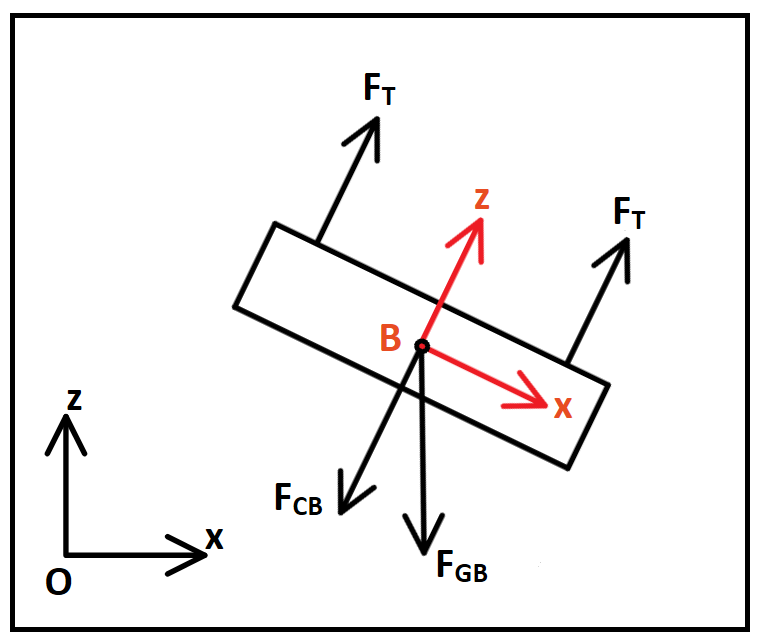
\includegraphics[width=0.7\textwidth]{./Wilson_img/B_mm.png}
\caption{Free-Body diagram of Body}
\end{figure}
Forces and Torques:
\begin{align*}
  \prescript{B}{}{\bm{F_{T}}} &=
  \begin{bmatrix}
    0 \\ 0 \\ F_{TB}
  \end{bmatrix} \\
  \prescript{O}{}{\bm{F_{GB}}} &=
  \begin{bmatrix}
    0 \\ 0 \\ -m_b g
  \end{bmatrix} \\
  \prescript{O}{}{\bm{F_{CB}}} &=
  \begin{bmatrix}
    F_{CBx} \\ F_{CBy} \\ F_{CBz} 
  \end{bmatrix} \\
  \prescript{B}{}{\bm{\tau_{CB}}} &=
  \begin{bmatrix}
    \tau_{CBx} \\ \tau_{CBy} \\ -\tau_{M} 
  \end{bmatrix}
\end{align*}

Net Force and Torque
\begin{align}
  \prescript{O}{}{\bm{F_{net,B}}} &= \prescript{O}{}{\bm{F_{GB}}} + \prescript{O}{}{\bm{F_{T}}} + \prescript{O}{}{\bm{F_{CB}}} = m_B \prescript{O}{}{\bm{a_B}} \\
  \prescript{O}{}{\bm{\tau_{net,B}}} &= R(\bm{q_B})\prescript{B}{}{\bm{\tau_{CB}}} = \prescript{O}{}{I_B} \prescript{O}{}{\bm{\alpha_B}}
\end{align}

\subsection{Controller Dynamics}
\begin{figure}[H]
\centering
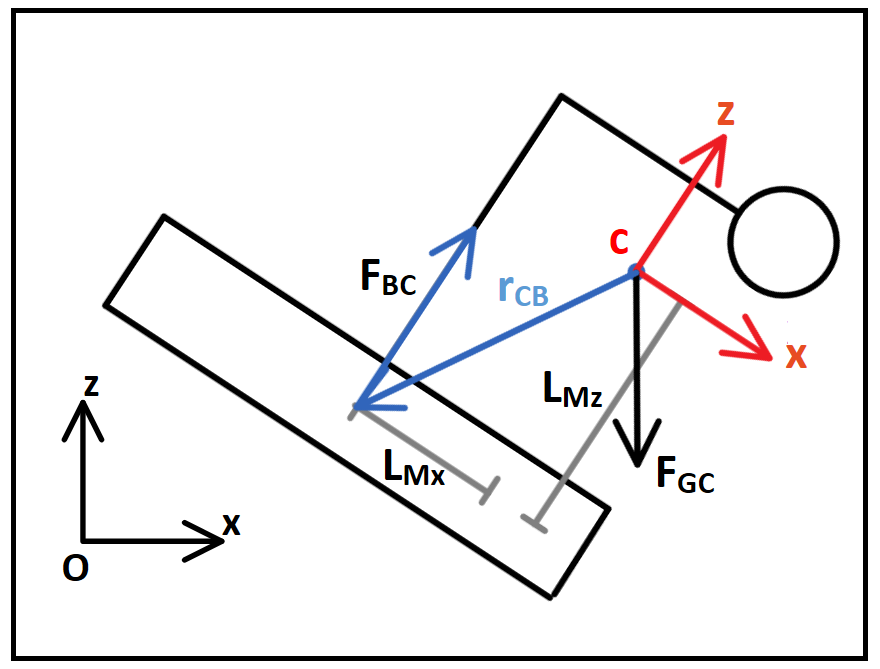
\includegraphics[width=0.7\textwidth]{./Wilson_img/C_mm.png}
\caption{Free-Body diagram of Controller}
\end{figure}
Forces and Torques:
\begin{align*}
  \prescript{O}{}{\bm{F_{BC}}} &=
  \begin{bmatrix}
    F_{BCx} \\ F_{BCy} \\ F_{BCz}
  \end{bmatrix} \\
  \prescript{O}{}{\bm{F_{GC}}} &=
  \begin{bmatrix}
    0 \\ 0 \\ -m_c g
  \end{bmatrix} \\
  \prescript{C}{}{\bm{\tau_{BC}}} &=
  \begin{bmatrix}
    \tau_{BCx} \\ \tau_{BCy} \\ \tau_{M} 
  \end{bmatrix} \\
  \prescript{O}{}{\bm{r_{CB}}} &= R(\bm{q_C}) \begin{bmatrix}
                                   -L_{Mx} \\ 0 \\ -L_{Mz}
                                 \end{bmatrix} \\
  \prescript{O}{}{\bm{\tau_{RF}}} &=  \prescript{O}{}{\bm{r_{CB}}} \times \prescript{O}{}{\bm{F_{BC}}}
\end{align*}
Net Force and Net Torque:
\begin{align}
  \prescript{O}{}{\bm{F_{net, C}}} &= \prescript{O}{}{\bm{F_{BC}}} + \prescript{O}{}{\bm{F_{GC}}} = m_C \prescript{O}{}{\bm{a_C}} \\
  \prescript{O}{}{\bm{\tau_{net, C}}} &= R(\bm{q_C})\prescript{C}{}{\bm{\tau_{BC}}} + \prescript{O}{}{\bm{\tau_{RF}}} = \prescript{O}{}{I_c} \prescript{O}{}{\bm{\alpha_C}}
\end{align}
\subsection{Constraints and Manipulation}
In the derivation below, assume everything is in the inertial frame unless explicitly stated. \par
The two bodies are contrainted (attached together), there are some relationship between the states and the forces between the body and the controller, 
\begin{align}
  \intertext{Let $\bm{p_{sys}} = \bm{p_B}$ and $\bm{q_{sys}} = \bm{q_{B}}$,}
  \begin{bmatrix}
    \bm{p_C} \\
    \bm{q_C}
  \end{bmatrix} &=
  \begin{bmatrix}
    \bm{p_B} + \bm{r_{BC}} \\
    \bm{q_{\theta}}\bm{q_B}
  \end{bmatrix}
  =
  \begin{bmatrix}
    \bm{p_{sys}} + \bm{r_{BC}} \\
    \bm{q_{\theta}}\bm{q_{sys}}
\end{bmatrix}  \\
% First Derivative
  \begin{bmatrix}
    \bm{\dot{p}_C} \\
    \bm{\dot{q}_C}
  \end{bmatrix} &=
  \begin{bmatrix}
    \bm{\dot{p}_{sys}} + \dot{R}(\bm{q_{sys}})\prescript{B}{}{\bm{r_{BC}}} \\
    \bm{q_{\theta}}\bm{\dot{q}_{sys}} + \bm{\dot{q}_{\theta}}\bm{q_{sys}} 
\end{bmatrix} \\
% Second Derivative
  \begin{bmatrix}
    \bm{\ddot{p}_C} \\
    \bm{\ddot{q}_C}
  \end{bmatrix} &=
  \begin{bmatrix}
    \bm{\ddot{p}_{sys}} + \ddot{R}(\bm{q_{sys}})\prescript{B}{}{\bm{r_{BC}}} \\
    \bm{q_{\theta}}\bm{\ddot{q}_{sys}} + 2[\bm{\dot{q_\theta}} \bm{\dot{q}_{sys}}] + \bm{\ddot{q}_{\theta}}\bm{q_{sys}} 
  \end{bmatrix} \\   
  \intertext{Newton's Third Law}
  \prescript{O}{}{\bm{F_{BC}}} &= -\prescript{O}{}{\bm{F_{CB}}} \\
  \prescript{O}{}{\bm{\tau_{BC}}} &= -\prescript{O}{}{\bm{\tau_{CB}}}
\end{align}
To limit our degree of freedom in the system, we have set a constraint for our quaternions, namely unit quaternion:
\begin{align}
  q_r^2 + q_i^2 + q_j^2 + q_k^2 = 1 \\
  q_r\dot{q_r} + q_i\dot{q_i} + q_j\dot{q_j} + q_k\dot{q_k} = 0\\
  q_r\ddot{q_r} + q_i\ddot{q_i} + q_j\ddot{q_j} + q_k\ddot{q_k} + \dot{q_r}^2 + \dot{q_i}^2 + \dot{q_j}^2 + \dot{q_k}^2 = 0
\end{align}
Last but not least, in the derivation below we use $\bm{q_\theta}$ directly for ease of typsetting, however, $q_{\theta}$ is not our state variable but $\theta$, their relationship is defined below,
\begin{figure}[H]
\centering
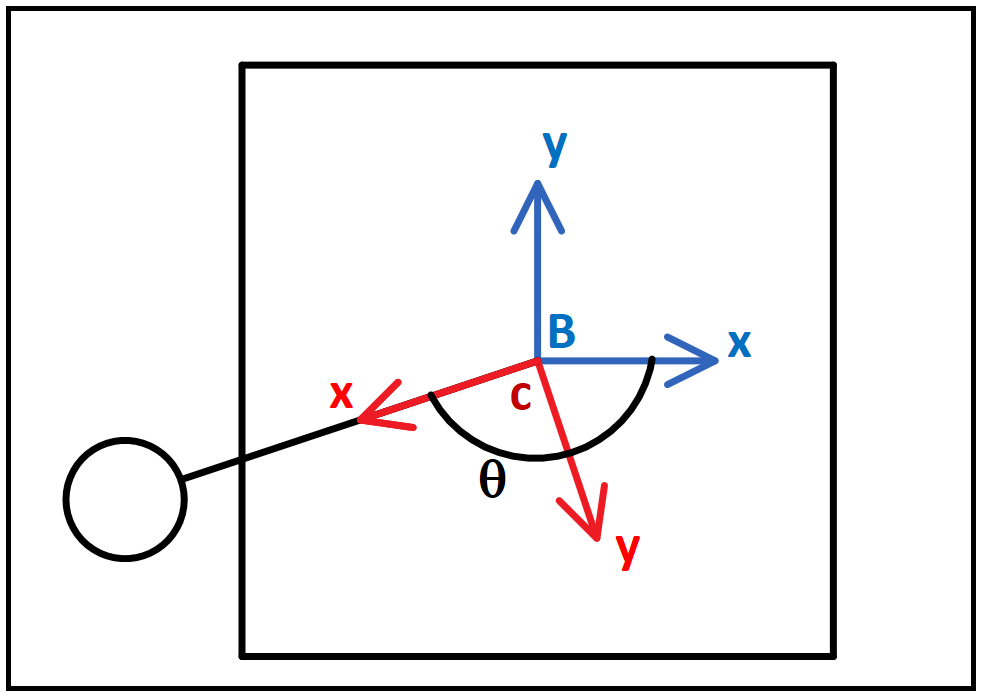
\includegraphics[width=0.7\textwidth]{./Wilson_img/qt_mm.png}
\caption{The yaw angle difference between Body and  Controller}
\end{figure}
\begin{align*}
  \bm{q_\theta} &= \cos(\frac{\theta}{2}) + \sin(\frac{\theta}{2})R(\bm{q_{sys}})\prescript{B}{}{\bm{\hat{z_B}}} \\
  \bm{\dot{q}_\theta} &= -\frac{1}{2}\sin(\frac{\theta}{2})\dot{\theta} + \frac{1}{2}\cos(\frac{\theta}{2})\dot{\theta}R(\bm{q_{sys}})\prescript{B}{}{\bm{\hat{z_B}}} + \sin{(\frac{\theta}{2})}\dot{R(\bm{q_{sys}})} \prescript{B}{}{\bm{\hat{z_B}}}
\end{align*}
where $\prescript{B}{}{\bm{\hat{z_B}}} =
\begin{bmatrix}
    0\\ 0\\ 1
\end{bmatrix}
$
\subsubsection{Combining the Force equations}
\begin{align*}
  \shortintertext{From (1),}
  \prescript{O}{}{\bm{F_{CB}}} &= m_B \prescript{O}{}{\bm{a_B}} - \prescript{O}{}{\bm{F_{GB}}} - \prescript{O}{}{\bm{F_{T}}} \\
  \shortintertext{From (3),}
  \prescript{O}{}{\bm{F_{BC}}} &= m_C \prescript{O}{}{\bm{a_C}} - \prescript{O}{}{\bm{F_{GC}}} \\
  \shortintertext{Using (6),}
  m_B \prescript{O}{}{\bm{a_B}} + m_C \prescript{O}{}{\bm{a_C}} &= \prescript{O}{}{\bm{F_{GC}}} + \prescript{O}{}{\bm{F_{GB}}} + \prescript{O}{}{\bm{F_{T}}} 
\end{align*}
Simplifying the above expression, we get
\begin{equation}
    (m_b + m_c) \bm{\ddot{p}_{sys}} + m_c \ddot{R}(\bm{q_{sys}}) \prescript{B}{}{\bm{r_{BC}}} = \bm{F_{GC}} + \bm{F_{GB}} + \bm{F_{T}} 
\end{equation}
\subsubsection{Combining the Torqe equations}
\begin{align*}
  \shortintertext{From (2),}
  \prescript{O}{}{\bm{\tau_{CB}}} &= \prescript{O}{}{I_B} \prescript{O}{}{\bm{\alpha_B}} \\
  \shortintertext{From (4),}
  \prescript{O}{}{\bm{\tau_{BC}}} &= \prescript{O}{}{I_c} \prescript{O}{}{\bm{\alpha_C}} - \prescript{O}{}{\bm{\tau_{RF}}}  \\
  \shortintertext{Using (7),}
  \prescript{O}{}{I_B} \prescript{O}{}{\bm{\alpha_B}} + \prescript{O}{}{I_c} \prescript{O}{}{\bm{\alpha_C}} &= \prescript{O}{}{\bm{\tau_{RF}}} \\
\end{align*}  
Assuming all the vectors are represented in the inertial O frame, using the quaternion representation for angular acceleration,
\begin{equation}
  I_B 2\left[\bm{\ddot{q}_B}\bm{q_B^*} - (\bm{\dot{q}_B} \bm{q_B^*})^2\right] + I_c 2 \left[\bm{\ddot{q}_C}\bm{q_C^*} - (\bm{\dot{q}_C} \bm{q_C^*})^2\right] = \prescript{O}{}{\bm{\tau_{RF}}}
\end{equation}
Substituting (5)-(7) in the above expression and isolating second derivative on the left, we have
\begin{align}
  2 I_B [\bm{\ddot{q}_{sys}} \bm{q_{sys}^*}] + 2I_C [\bm{q_{\theta}}\bm{\ddot{q}_{sys}} (\bm{q_{\theta}} \bm{q_{sys}})^{\bm{*}}] + 2 I_C [\bm{\ddot{q}_{\theta}} \bm{q_{sys}}](\bm{q_{\theta}q_{sys}})^{\bm{*}} - \bm{r_{CB}} \times \bm{F_{BC}} = \zeta
\end{align}
where
\begin{align*}
  \zeta = 2I_B(\bm{\dot{q}_{sys}}\bm{q_{sys}^*})^2 + 2I_C[(\bm{q_\theta} \bm{\dot{q}_{sys}} + \bm{\dot{q}_\theta}\bm{q_{sys}})(\bm{q_{\theta}\bm{q_{sys}}})^{\bm{*}}]^2 - 4I_C(\bm{\dot{q}_{\theta}\dot{q}_{sys}} )(\bm{q_\theta q_{sys}})^{\bm{*}}
\end{align*}
Note that we put $\bm{\tau_{RF}}$ on the left hand side, this is because we can express $\bm{F_{BC}}$ in terms of $\bm{\ddot{p}_{sys}}$ from (1), a second derivative of positional state
\begin{align*}
  \bm{F_{BC}} = m_B \bm{\ddot{p}_{sys}} - \bm{F_{GB}} - \bm{F_{T}}
\end{align*}

\subsection{System of equations}
From equation (12), (14), and (15), we have the function that relates our state variables together,
\begin{align}
  f(\bm{\ddot{p}},\bm{\ddot{q}}, \ddot{\theta}, \bm{\dot{p}},\bm{\dot{q}}, \dot{\theta},\bm{p},\bm{q}, \theta) = 0
\end{align}
Assuming we can solve for $\bm{\ddot{p}},\bm{\ddot{q}}, \ddot{\theta}$ given $\bm{\dot{p}},\bm{\dot{q}}, \dot{\theta},\bm{p},\bm{q}, \theta$, let the state of our system to be
\begin{align*}
  \bm{s_{sys}} =
  \begin{bmatrix}
      \bm{\dot{p}} \\
      \bm{\dot{q}} \\
      \dot{\theta} \\
      \bm{p} \\
      \bm{q} \\
      \theta
  \end{bmatrix}
  \quad \text{so that} \quad
  \bm{\dot{s}_{sys}} =
    \begin{bmatrix}
      \bm{\ddot{p}} \\
      \bm{\ddot{q}} \\
      \dot{\ddot\theta} \\
      \bm{\dot{p}} \\
      \bm{\dot{q}} \\
      \dot{\dot{\theta}}
  \end{bmatrix}
\end{align*}
We have our state evolution equations as
\begin{align}
  s_{t+1} = s_{t} + \dot{s}_{t}\Delta t
\end{align}

\subsection{Matlab Implementation}
Implementing the systems of equations in (16), and solve for $\bm{\ddot{p}},\bm{\ddot{q}}, \ddot{\theta}$ given $\bm{\dot{p}},\bm{\dot{q}}, \dot{\theta},\bm{p},\bm{q}, \theta$ in Matlab doesn't yield a solution. There must be something wrong with the equations / the implementation.
\section{Simulation}
\subsection{The goals of simulation}
Before starting the real-world implementation, we decided to make a dynamic 3D simulation of the quadcopter with spinning mass to visualize the motion of it and get a better understanding of the specific behavior of such a quadcopter.
\newline
\newline
We set three main goals for the 3D simulation. First, we want to see a 3D graphic model for the quadcopter with as many details as possible. Second, using our knowledge of physics and math, we want to describe the motion of the quadcopter to be as close to the real-world-motion as possible in the 3D simulation world. Third, we want to obtain as many useful parameters and insights as possible from the simulation so that we can apply them in the real implementation.
\subsection{Building 3D structure}
The first thing we did was to measure every possible dimension of the quadcopter and sketch the corresponding geometric figure of it. Then we tried to decompose the entire geometric figure with several typical geometric components such as cylinder, sphere etc.
\begin{figure}[h]
\centering
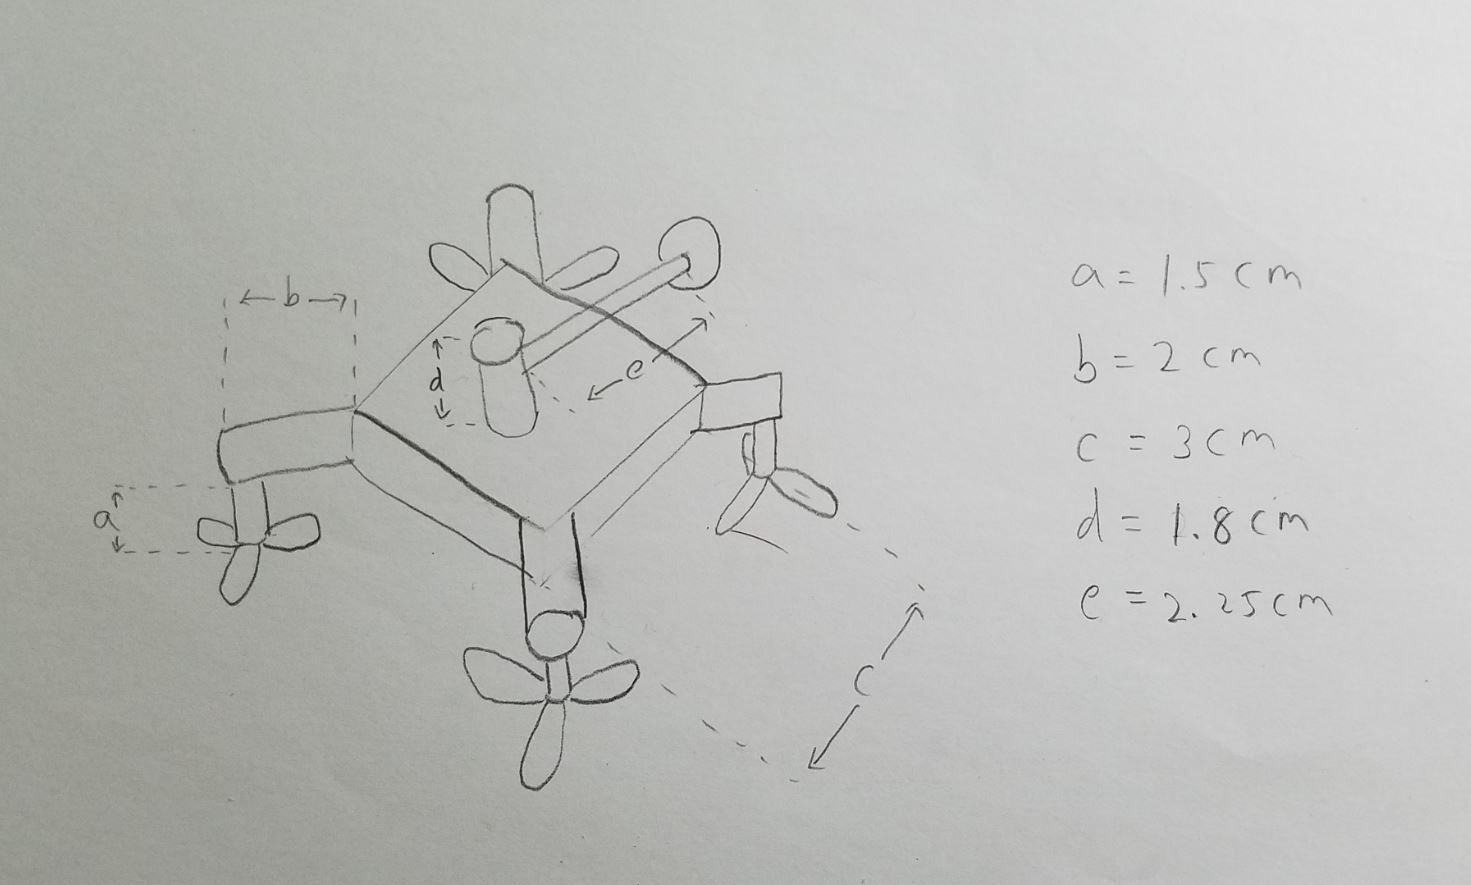
\includegraphics[width=0.7\textwidth]{./Lin_img/0.jpg}
\caption{The rough sketch of the quadcopter}
\end{figure}
\begin{center}
\begin{tabular}{ |p{3cm}|p{3cm}|p{3cm}|  }
 \hline
 \multicolumn{3}{|c|}{Geometric Components} \\
 \hline
 Name   & Shape   &Amount \\
 \hline
 Main Body & Box & 1  \\
 Motor & Cylinder & 1  \\
 Mass Stick    & Cylinder & 1 \\
 Mass &  Sphere & 1 \\
 Leg & Cylinder & 4  \\
 Propeller Holder & Cylinder & 4  \\
 Propeller & Propeller & 4  \\
 \hline
\end{tabular}
\end{center}
The reason why we used the typical geometric components is that they can be easily defined in the 3D editor. In the 3D editor, we had to build the 3D quadcopter structure piece by piece. And if we can define each piece with the simple geometric shape, then we can just try to combine them together properly to get the whole 3D structure.
\newline
\newline
As it’s been mentioned, we used Simulink’s 3D world editor to build the 3D geometric structure for the quadcopter. There’re two important things I’d like to mention about the 3D world editor. 
\newline
\newline
First, its parent-children relationship tree. Each geometric component of the structure plays a role as either a parent or a child or both in the relationship tree. For example, a leg of the quadcopter is the parent component of the propeller and at the same time it’s the child component of the main body.
\begin{figure}[h]
\centering
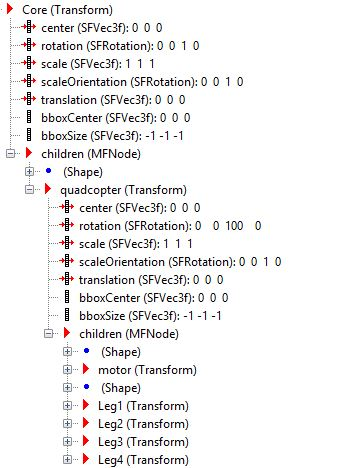
\includegraphics[width=0.6\textwidth]{./Lin_img/1.JPG}
\caption{The parent-children relationship tree}
\end{figure}
\newline
When the parent component is changing its state, all its children components and its grandchildren components will also change their reference frame and origin with it. However, when a child component is changing its state, it will not effect on either the parent or other sibling children components. This is similar with the joints of an robotic arm, the (n)th joint will effect on the (n+1)th joint, but (n+1)th joint won’t effect on its previous joint -- (n)th joint.
\newline
\newline
Second, its state representation system. The 3D world editor is using the Axis-Angle representation(quaternion representation) for its rotational state representation. 
\begin{figure}[h]
\centering
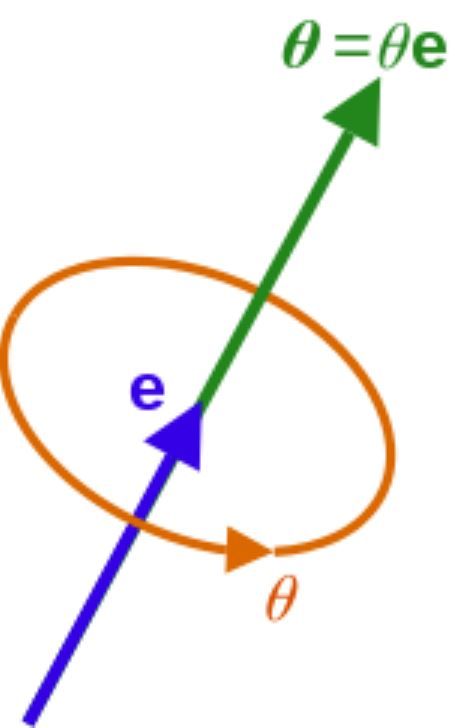
\includegraphics[width=0.3\textwidth]{./Lin_img/2.JPG}
\caption{The Axis-Angle representation}
\end{figure}
\newline 
Basically, it uses a 4-vector to represent the rotational state. The first 3 entries of the vector represent the x,y,z component of the rotating axis direction(vector (e) in the figure), and the fourth entry represents the angle(theta in the figure) that the corresponding object has been rotated due to the rotating axis.
\newline
\newline
For the translational state, it uses the normal Cartesian coordinate system representation. It has a 3-vector with each of the entry represents x,y,z component in the cartesian coordinate system. 
\newline
\newline
In other words, each of the geometric piece has up to 7 entries(4 from the rotational state, 3 from the translational state) that can be updated in each cycle of the 3D frame generating.
\newline
\newline
We had to initialize these 7 states for each of the geometric component one by one. We started with the core of the quadcopter. The core can be understood as the geometric center of the main body of the quadcopter. Then we added the main body as the child of the core. The motor and the four legs were added as the children of the main body, the mass stick and the mass were added as the child and the grandchild of the motor. 
\newline
\newline
And finally, the propeller holders and the propellers were added as the children and the grandchildren of the legs. In this way, we finished building the 3D geometric structure of our quadcopter as it can be seen in the figure.

\begin{figure}[h]
\centering
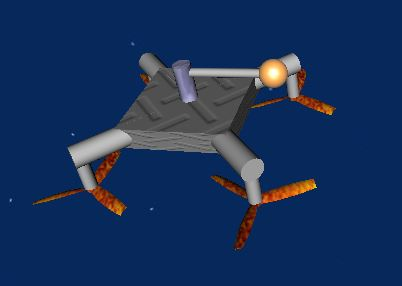
\includegraphics[width=0.7\textwidth]{./Lin_img/3.JPG}
\caption{The completed quadcopter 3D model}
\end{figure}


\subsection{Creating dynamic 3D simulation}
After building the 3D model of the quadcopter, we started creating the dynamic 3D simulation using Simulink blocks. We embedded the 3D structure we built into the block VR sink. 
\newline
\newline
When we run the Simulink program, in each unit time cycle, the VR sink block will generate one 3D frame according to the current state of the 3D structure in it. 
\newline
\newline
So if we can update the state of the 3D structure, we can obtain a dynamic 3D simulation from it. The state of the 3D structure in the VR sink block can be updated through the namely “state updating windows”.As it can be seen in the figure, there are some arrows pointing at "windows" called "Core.translation", "motor.rotation" etc. For example, we can use the window called "Core.translation" to update the translational state of the core of the quadcopter.
\begin{figure}[h]
\centering
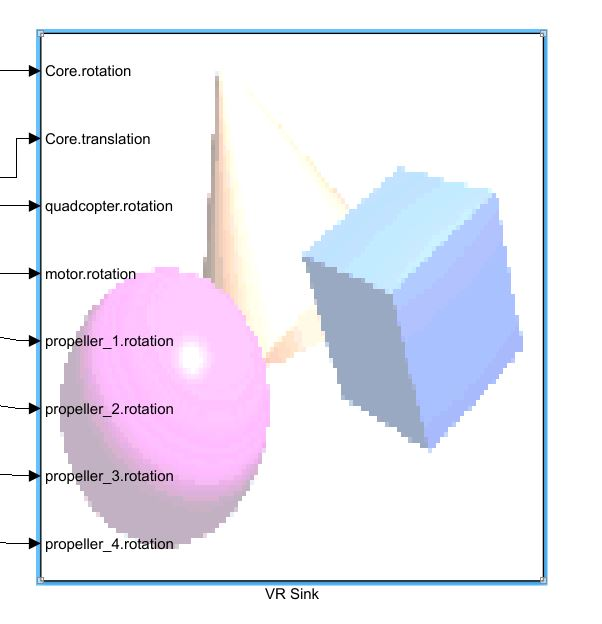
\includegraphics[width=0.6\textwidth]{./Lin_img/4.JPG}
\caption{The VR sink block and the state updating windows}
\end{figure}
\newline
Before updating any state, we had to determine exactly how many and which states from which geometric components we’d like to update with the state updating windows. 
\newline
\newline
We have 4 rotating propellers attached on the legs, 1 rotating arm(or motor) on the top of the quadcopter, and the main body of the quadcopter will also rotate, the core of the entire quadcopter will be rotating and translating.
\newline
\newline
Therefore, in order to obtain a realistic simulation, we needed to update 6 rotational states and 1 translational state. And each of the rotational state had to be updated using a 4-vector data and the translational state had to be updated using a 3-vector data.
So we added 7 state updating windows on the VR sink block with the proper Simulink block settings.
\newline
\newline
Apparently, the most important states among the 7 states we chose are the translational and rotational states of the core. Because they are the states that can be used to describe the overall movement of the quadcopter. 
\newline
\newline
Other states, such as the rotational state of the propellers are just for creating more realistic animation, so they just needed to be set up with a reasonable constant as its rotating speed. 
\newline
\newline
In this simulation, we were assuming that the relative positions of the propellers are perfectly symmetric and the thrust force from each of them is exactly the same so that there’s a constant thrust force that is applied at right on the center of the core.
\begin{figure}[h]
\centering
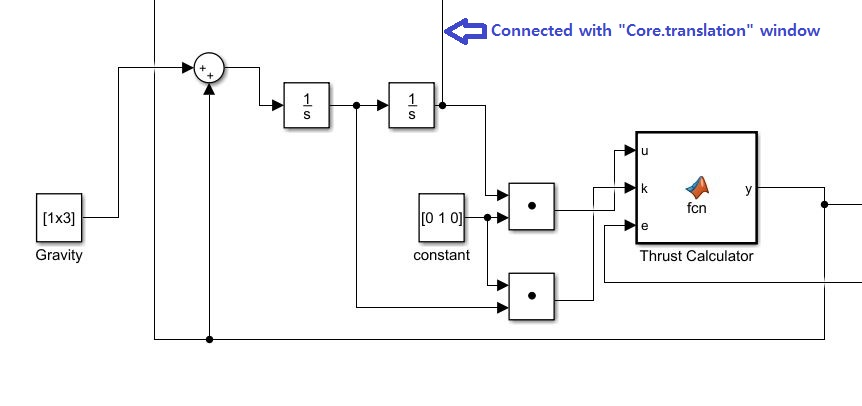
\includegraphics[width=1.1\textwidth]{./Lin_img/5.JPG}
\caption{The translational acceleration calculating system}
\end{figure}
\newline
The direction and the amplitude of that thrust force will be calculated in the thrust calculator block in each unit time cycle and the result will be used to update the translational state of the core.
\newline
\newline
Other than that, the main role of the translational acceleration calculating system is to add the translational acceleration which come from the thrust force and gravitational force and use that to update the translational state of the core. The translational state has only 3 DOF and they can be fully described by this translational acceleration  calculating system.
\newline
\newline
For the rotational state, however, unfortunately we don’t have any complete math model to fully describe all situations. So we had to make assumptions that can limit the complexity of the motion. 
\begin{figure}[h]
\centering
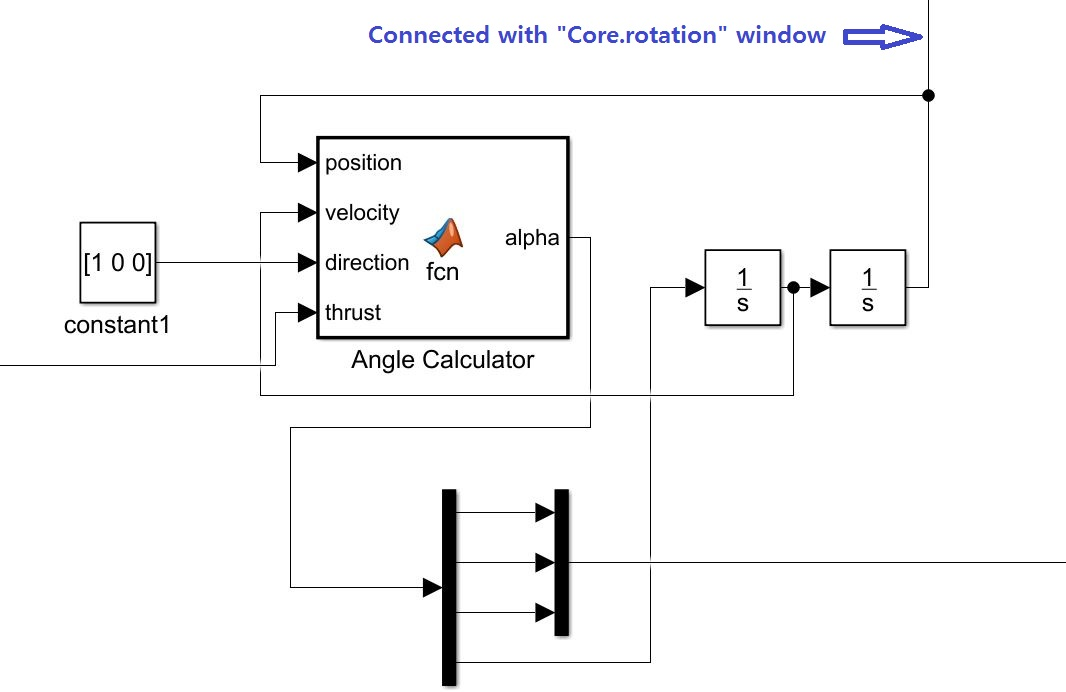
\includegraphics[width=1.0\textwidth]{./Lin_img/6.JPG}
\caption{The rotational acceleration calculating system}
\end{figure}
\newline
We assumed that we already have the perfect control method for the spinning mass that is we can let the mass stay at one position as long as we want and we can move it to another position instantly.
\newline
\newline
For example, suppose the full range of the spinning mass is from 0 degree to 360 degree, we let it stay at 0 degree for a certain period of time and then let it move to 180 degree position instantly and stay there for a certain period of time and then move back to 0 degree position instantly and so on. 
\newline
\newline
In this way, the overall center of mass will always stay in one plane, shifting back and forth so that we can fully describe it by updating the 4-vector of the rotational state of the core.
\newline
\newline
Under such assumptions, the rotational acceleration calculating system will use the information of the current state to calculate the rotational state for the next cycle and update it through the state updating window for the rotational state of the core.
\newline
\newline
In this way, with the help of other blocks and the proper connections, the translational and rotational acceleration calculating systems can work together to generate the updated state information for each geometric component of the 3D quadcopter model in each time cycle so that we can see a continuous, realistic dynamic simulation when we run the program. For the simulation demo videos and more details, please check our \href{https://github.com/Amir-Omidfar/183DB-}{Github repo}.
\begin{figure}[h]
\centering
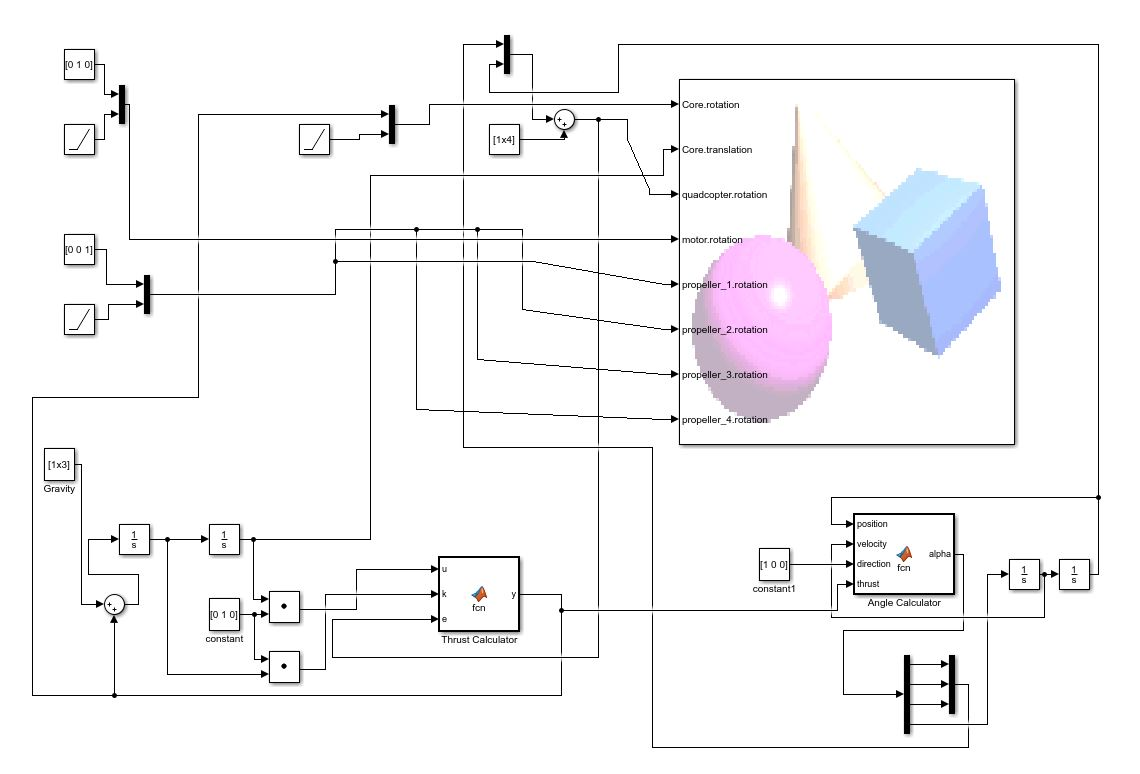
\includegraphics[width=0.9\textwidth]{./Lin_img/7.JPG}
\caption{The completed simulink block diagram}
\end{figure}
\newline
\subsection{Obtaining parameters and insights}
As it can be seen in the simulation demo video, we achieved most of our goals for the simulation part pretty well. We built a decent 3D structure for the quad-copter. Though our knowledge of physics and math is limited to derive the complete solution for the motion, we made assumptions under which we can build a simulation model that is as close to the reality as possible. 
\newline
\newline
And finally, we also expected to get some useful parameters and insights that we can apply in the real implementation. The parameters that are mentioned in this section are obtained experimentally by trying different values one by one and observing the behavior of the quad-copter in the simulation.
\newline
\newline
The first parameter we were interested in was the spinning rate of the arm. When we set it up to be a very small number, in other words if the mass stays at one position for too long time, the quad-copter gets flipped over very soon after running the simulation. 
\begin{figure}[h]
\centering
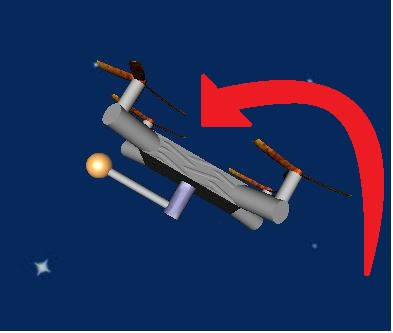
\includegraphics[width=0.6\textwidth]{./Lin_img/8.JPG}
\caption{The quad-copter gets flipped over}
\end{figure}
\newline
And when we set it up to be larger and larger number, we noticed that it takes longer and longer until it gets flipped over. And when the rate is going over about 10 cycles/second, the quad-copter seems to be very stable.
\newline
\newline
Due to the assumptions we made, the spinning rate value cannot be very reliable in this case, but it tells us the essential insight that until we can get a fast enough spinning rate for the arm, we will never get the quad-copter stable.
\newline
\newline
The next parameter we were interested in was the pitching angle. The pitching angle here is the angle it pitches by when it’s moving towards a certain direction.
\newline
\newline
We realized that if we set this angle too large, the quad-copter will get flipped easily, and if we set this angle too small, the quad-copter will not move towards a certain direction but wiggle at the same position.
\newline
\newline
After trying many different angles, we found that the pitching angle that has the best performance is about 22 degree measuring from the vertical axis that is pointing up.
\begin{figure}[h]
\centering
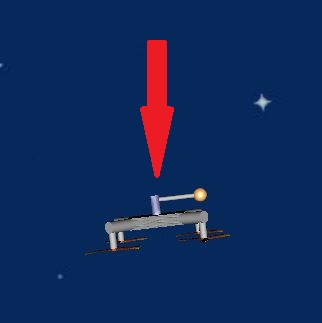
\includegraphics[width=0.5\textwidth]{./Lin_img/9.jpg}
\caption{The quad-copter falls down if the parameter is not appropriate}
\end{figure}
\newline
This value we obtained from the simulating experiment is supposed to be more reliable than the spinning rate we mentioned earlier. Because even though we assumed that the mass can move from one place to another instantly, that won’t effect on the accuracy of the optimal value of the pitching angle since the pitching direction is in the same plane with the positions that the mass is staying. 
\newline
\newline
It tells us that no matter where we let the mass stay, we should never let the pitching angle go over 22 degree on that specific direction, otherwise it will get flipped over.
\newline
\newline
Lastly, we expected to know how much thrust force would be enough to maintain a stable movement. We noticed that if the thrust force is too small, it will just keep falling, and if the thrust force is too large, it will either keep going up or get flipped over quickly. 
\begin{figure}[h]
\centering
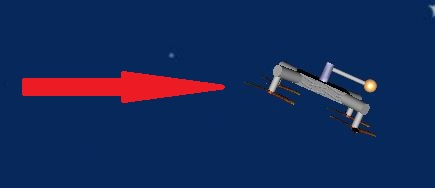
\includegraphics[width=0.8\textwidth]{./Lin_img/10.jpg}
\caption{The quad-copter with appropriate parameters}
\end{figure}
\newline
The ideal thrust force we found after trying many possible values was about 1.2G. 1G here represents the force that equals to the gravitational force that comes from the entire quad-copter. So for example, if the weight of the quad-copter is 10g, we need to provide a thrust force that equals to the gravitational force of a 12g object.
\newline
\newline
Similar with the pitching angle, this parameter for the thrust force also can be considered as a pretty reliable parameter, because again, the thrust force is in the same plane with the positions that the spinning mass is staying. Basically, any parameters that come from the same plane with the spinning mass is supposed to be reliable since their accuracy gets little influence from the assumption we made.
\newline
\newline
This was confirmed later in our real implementation, we designed the spinning arm using the weight limitation that was calculated based on the 1.2G thrust force parameter we obtained from the simulation. And when we tested it using different load, the quad-copter was behaving almost as the same as what we saw in the simulation. 
\section{Off center spinning module design}
In order to clarify the steps taken in designing the spinning mass module, we start with reviewing some main specifications of the quad-copter used for the purpose in the project.
\subsection{Quad-copter Specifications}
Crazyflie 2.0 is a 27 gram nano quad-copter used for this project. As for designing our spinning mass module, the main constraint was the maximum payload that Crazyflie could handle. According to Crazyflie 2.0 hardware specifications maximum recommended payload is 15 grams. Therefore the spinning mass module initially assumed to have maximum weight of 15 grams.
\begin{figure}[h]
\centering
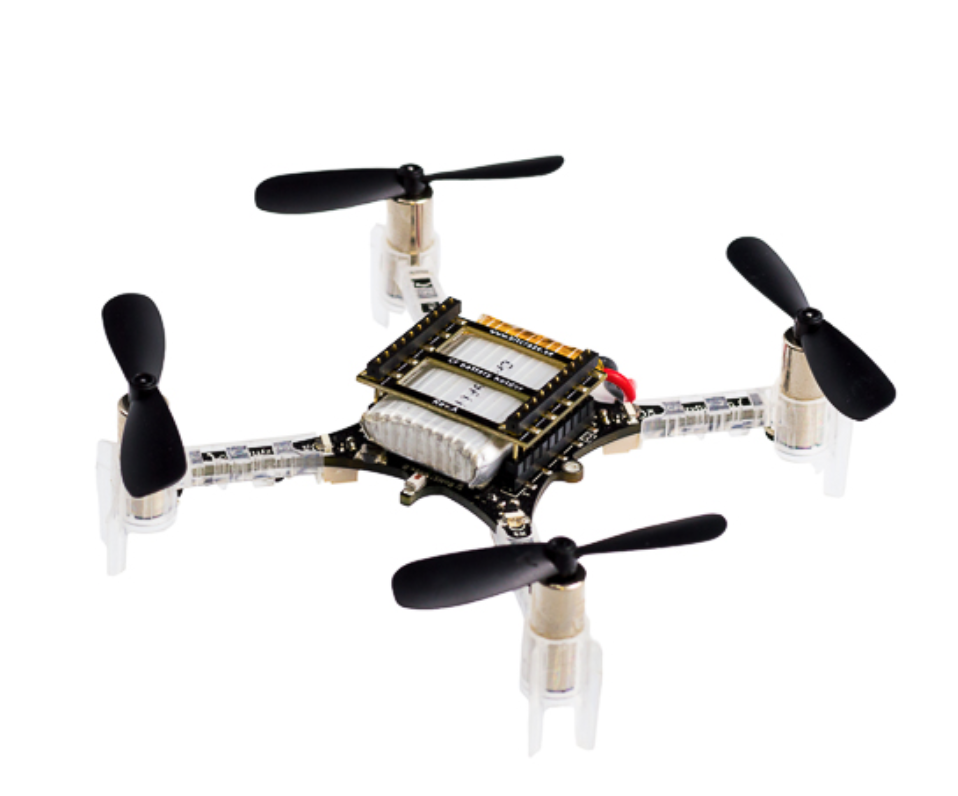
\includegraphics[width=0.5\textwidth]{./Amir_img/CF.png}
\caption{Crazyflie 2.0}
\end{figure}

\subsection{Spinning mass considerations}
Our design of spinning mass was consisted of selecting below components:
\begin{enumerate}
  \item DC motor
  \item Rotating arm and Spinning mass
  \item Rotary encoder 
\end{enumerate}
\subsubsection{DC motor}
As mentioned, mainly constrained by maximum payload for spinning mass module, we needed small, light motor with control feedback. Next important constraint was voltage and current criteria of the motor. Ideally we aimed to power the module from Crazyflie power supply which was 3.7V (250 mAh) battery. Adding external battery was not ideal for our weight limit, so before implementation we tested our candidate motor along with the quad-copter four motors and measured voltage and current drawn by selected motor. There we observed the selected motor would draw around 0.4 A spinning at sutiable range for our goal Consequently we selected the same type of DC motor as those utilized in the quad-copter. 
\begin{figure}[h]
\centering
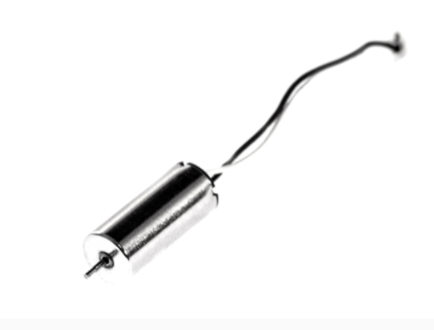
\includegraphics[width=0.5\textwidth]{./Amir_img/DCmotor.png}
\caption{7mm Core less DC motor}
\end{figure}
\newline 
Using the Selected 7x16 mm Core-less DC motor,we estimated the complete system (quad-copter and spinning mass module) to run for 4 minutes. We agreed this amount of time would be enough for demonstrations purposes at this point. Below is the specifications of the DC motor used.
\newline
\begin{center}
\begin{tabular}{ |p{3cm}|p{3cm}|  }
 \hline
 \multicolumn{2}{|c|}{Mechanical Specifications} \\
 \hline
 Diameter   & 7.0 mm    \\
 Length &   16.0 mm  \\
 Shaft length & 3.5 mm  \\
 Shaft diameter    & 0.8 mm \\
 Weight &   2.7g \\
 Wire length & 32.0 mm  \\
 \hline
 \multicolumn{2}{|c|}{Electrical Specifications} \\
 \hline 
 Kv & 14000 rpm/V \\
 Rated voltage & 4.2v \\
 Rated current & 1000mA\\
 \hline
\end{tabular}
\end{center}
  
\subsubsection{Rotating arm and Spinning mass}
Now we shall explain the design process of the rotating arm. 
Below is the initial design for rotating arm. 
\begin{figure}[h]
\centering
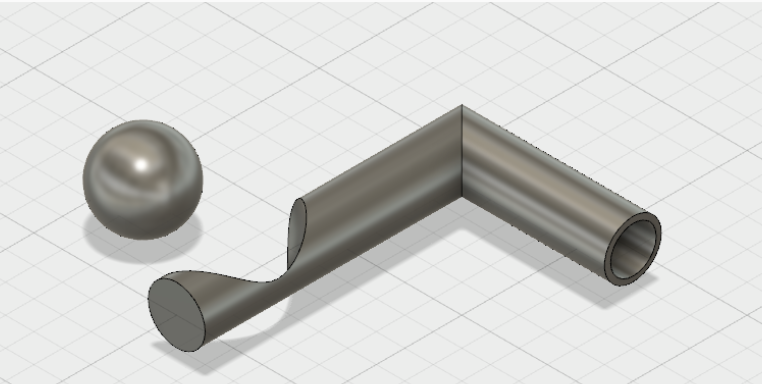
\includegraphics[width=0.5\textwidth]{./Amir_img/rotatingArm.png}
\caption{Rotating arm and spinning mass design}
\end{figure}
\newline
The arm length and height, considering the specifications of the quad-copter, were decided to be 5 cm and 3 cm respectively.The diameter of the cylindrical was 10 mm with 2mm thickness on sides to provide slightly larger gap than 7mm(motor diameter) with small hole where the motor can get attached to the rotating arm. 
\newline
Going back to our weight constraint. Our weight limit for rotating arm along with spinning mass was almost around 12 gram. (Explained in the table below)

\begin{center}
\begin{tabular}{ |p{6cm}|p{1cm}|  }
 \hline
 \multicolumn{2}{|c|}{Weight constraints} \\
 \hline
 Maximum payload   & 15 g   \\
 Motor weight &   2.7 g  \\
 Rotating arm and spinning mass & ? \\
 \hline
\end{tabular}
\end{center}

PLA filament with density of $1.25$ $g/cm^3$ was used for printing the rotating arm. The printed arm (shown in figure 7) weighted about $7$ grams, which limited our spinning mass weight to under 5 grams.($12-5=7 grams$)
\begin{figure}[h]
\centering
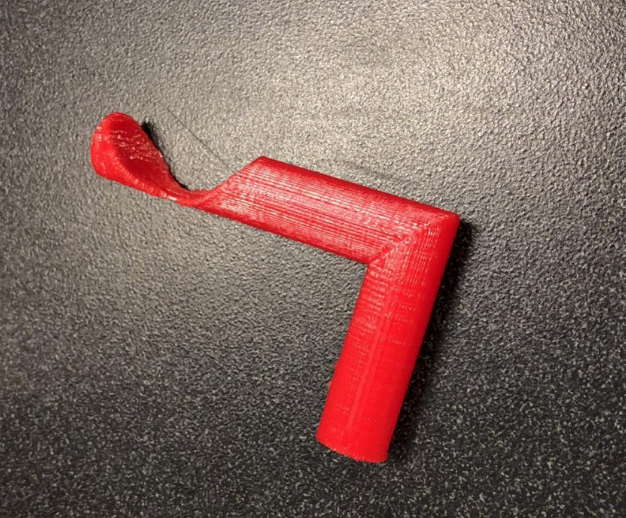
\includegraphics[width=0.5\textwidth]{./Amir_img/rotatingArm1.png}
\caption{Rotating arm}
\end{figure}

For spinning mass we used few different types of bolts (all lighter than 5 grams). Also we thought for final design an ideal case would be to use small precision ball bearings with weight range between 3-5 grams.(shown i figure 8)
\begin{figure}[h]
\centering
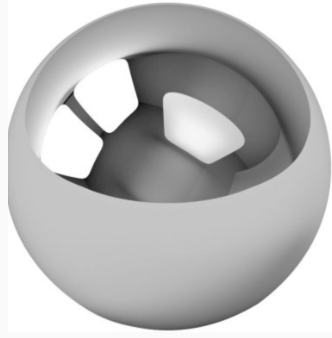
\includegraphics[width=0.25\textwidth]{./Amir_img/spinningMass.png}
\caption{ball bearing for spinning mass}
\end{figure}


\subsubsection{Rotary encoder }

In order to have better feedback of the system dynamics and to have more control over the angular velocity of rotating arm, we decided to add off-axis encoder.
\begin{figure}[H]
\centering
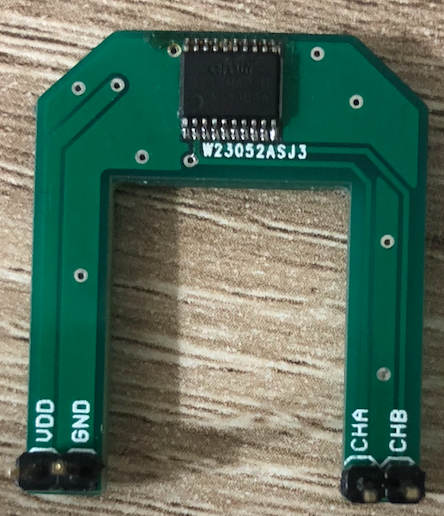
\includegraphics[width=0.25\textwidth]{./Amir_img/enc1.png}
\caption{Encoder}
\end{figure}

The rotary off axis encoder required us to redesign our rotating arm. We added an extra hole to place magnet on rotating arm and Styrofoam to hold our motor and the encoder on top of our quad-copter. 
\begin{center}
\begin{figure}[H]
\centering
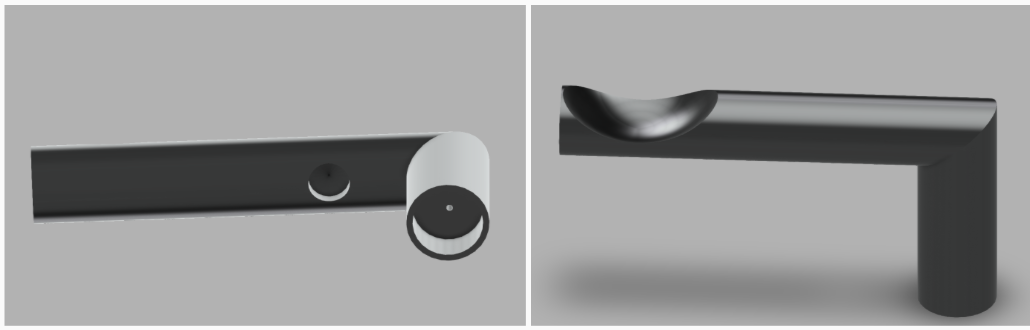
\includegraphics[width=1.0\textwidth]{./Amir_img/modifiedArm.png}
\caption{Modified rotating arm}
\end{figure}


\begin{figure}[H]
\centering
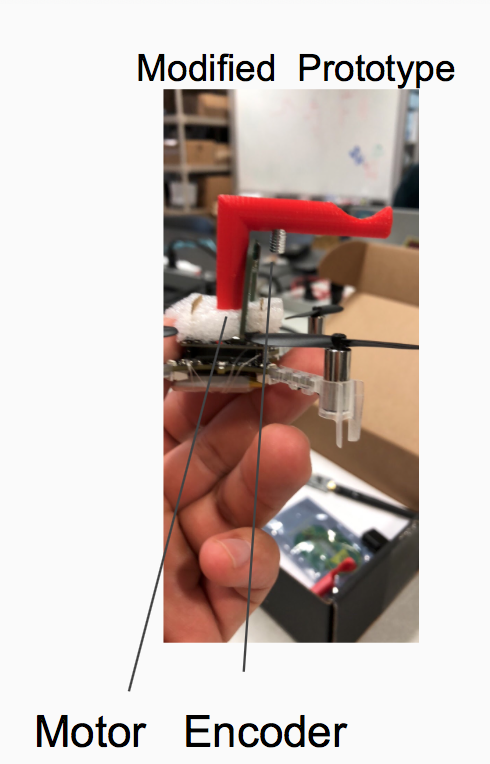
\includegraphics[width=0.5\textwidth]{./Amir_img/updatedController.png}
\caption{Spinning mass module with encoder on quad-copter}
\end{figure}
\end{center}





%%%%%%%%%%%%%%%%%%%%%%%%%%%% START OF MOTOR DRIVER SECTION %%%%%%%%%%%%%%%%%%
\section{Motor controller circuit}
Now with rotating arm components defined we move on to motor driver for spinning module controller. 
\subsection{PCB Design}
Initially we decided to design separate PCB that can be mounted on the quad-copter with its individual circuitry. For that purpose we created a list of components we required and made the schematics for our motor controller circuit. (Schematics file shown in figure below is attached with project files)
\newline

\begin{figure}[H]
\centering
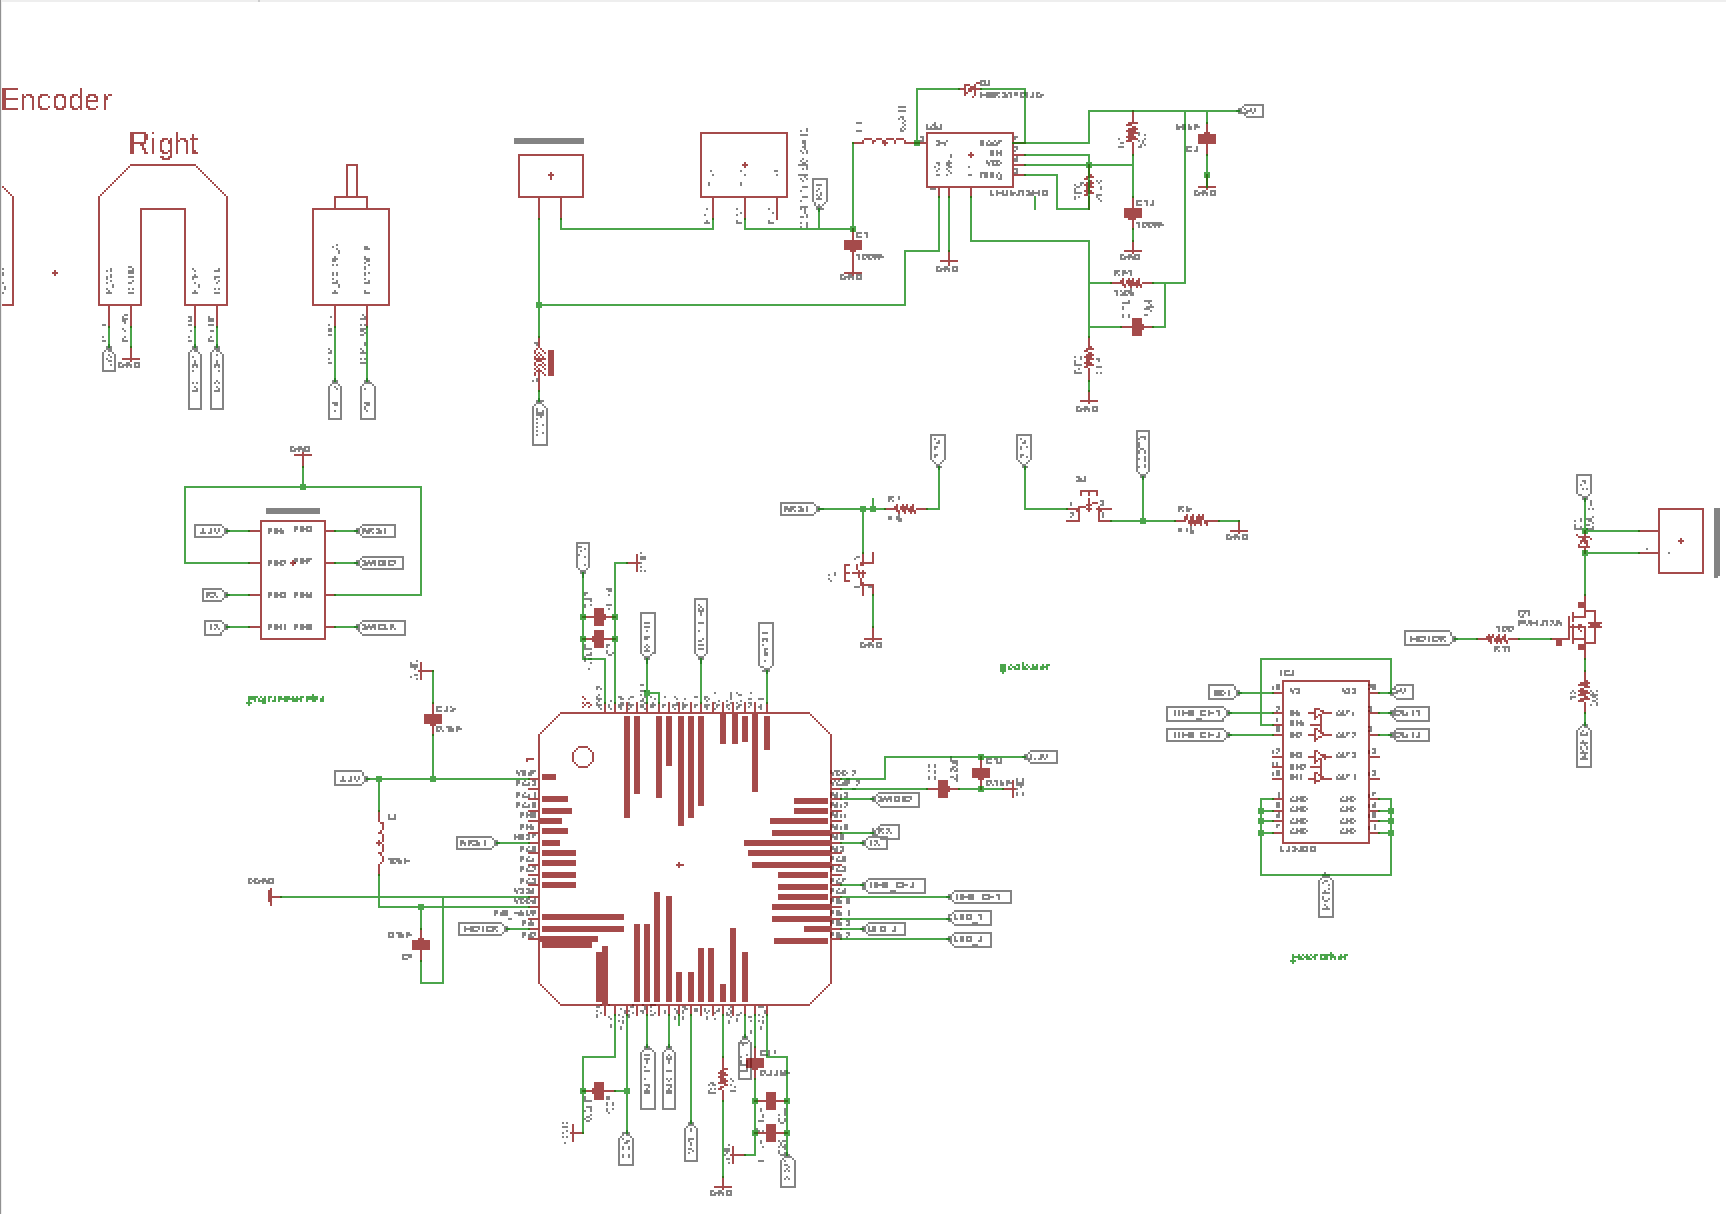
\includegraphics[width=0.5\textwidth]{./Amir_img/schematics.png}
\caption{Controller circuit Schematics}
\end{figure}

 Our initial schematics included all below surface mount components:
 
\begin{enumerate}
\item MCU
\item  Motor Driver
\item Voltage Regulator
\item DC motor and rotary encoder
\end{enumerate}
 
\subsubsection{MCU}
The micro-controller selected is STM32F405, a 32 bit MCU by STM. Possibly a controller with lower power and less computation power would have sufficed since there was no heavy computation in the encoder part of our circuit. However, the reason to select STM32F405 was mainly due to our prior experience with this chip and the fact that it was easy to program with programmable cable we had. 

\begin{figure}[H]
\centering
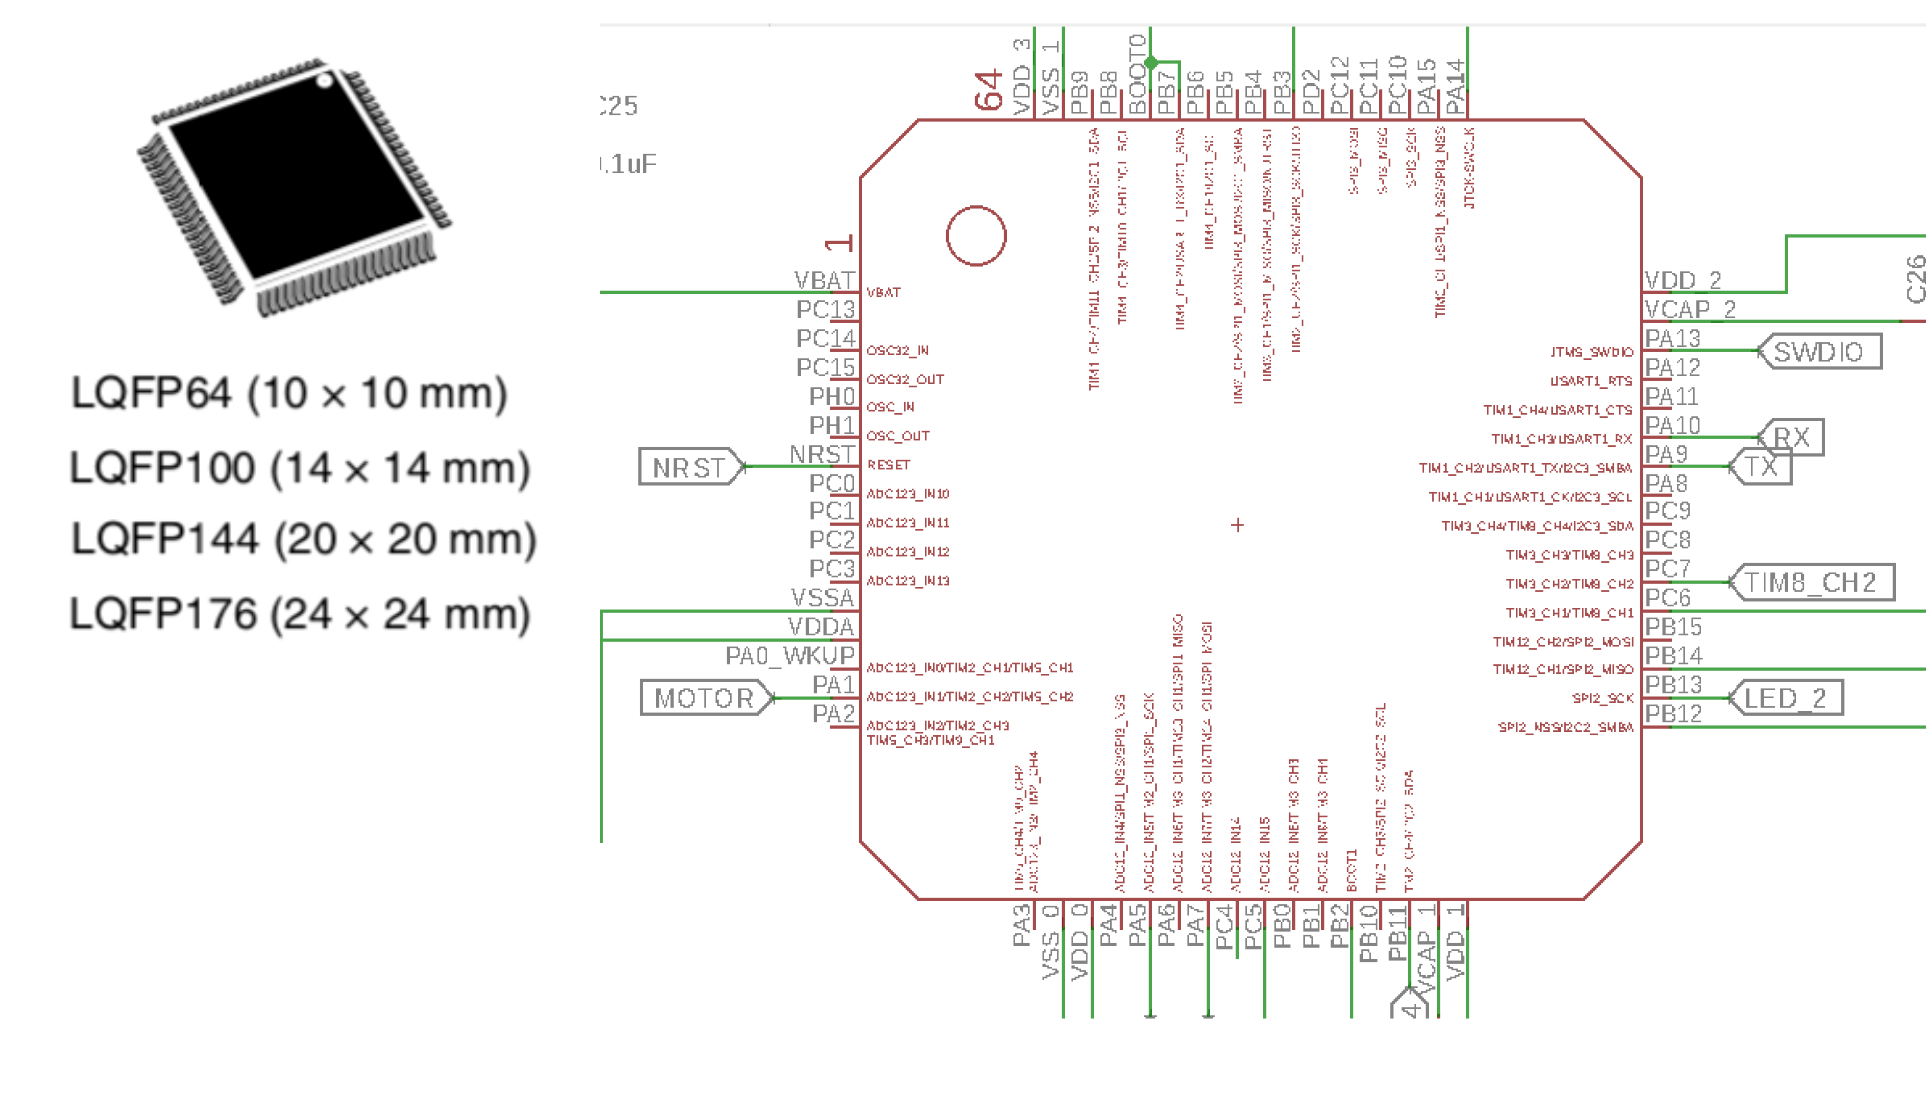
\includegraphics[width=1\textwidth]{./Amir_img/stmMcu.png}
\caption{MCU of the motor controller circuit}
\end{figure}

\subsubsection{Motor driver}
We designed two motor driver circuits for our spinning mass module. 
\begin{enumerate}
 \item Unidirectional motor driver: 
 Here in this motor driver the SMD N-channel Mosfet "irlml2502trpbf" acts as on/off switch which is ideally controlled by MCU through user's input. This driver given PWM signals was able to run the motor at different speeds only in one direction. 
\begin{figure}[H]
\centering
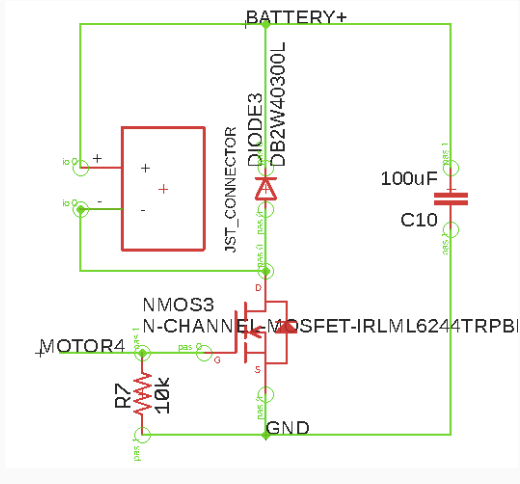
\includegraphics[width=0.5\textwidth]{./Amir_img/uniDriver.png}
\caption{schematics of the unidirectional motor driver}
\end{figure} 
 \item Bidirectional driver:
 Just like the case with encoder, in order to have more robust control over our spinning mass module, we decided to have bidirectional motor driver where moving in opposite directions could help to stabilize the very under-actuated system of our quad-copter. In this setup two separate PWM signals from MUC are input to H-bridge that determine the direction of rotation for spinning mass and its angular velocity. For this purpose, SMD version of L293DD was implemented as H-bridge. 
 \begin{figure}[H]
\centering
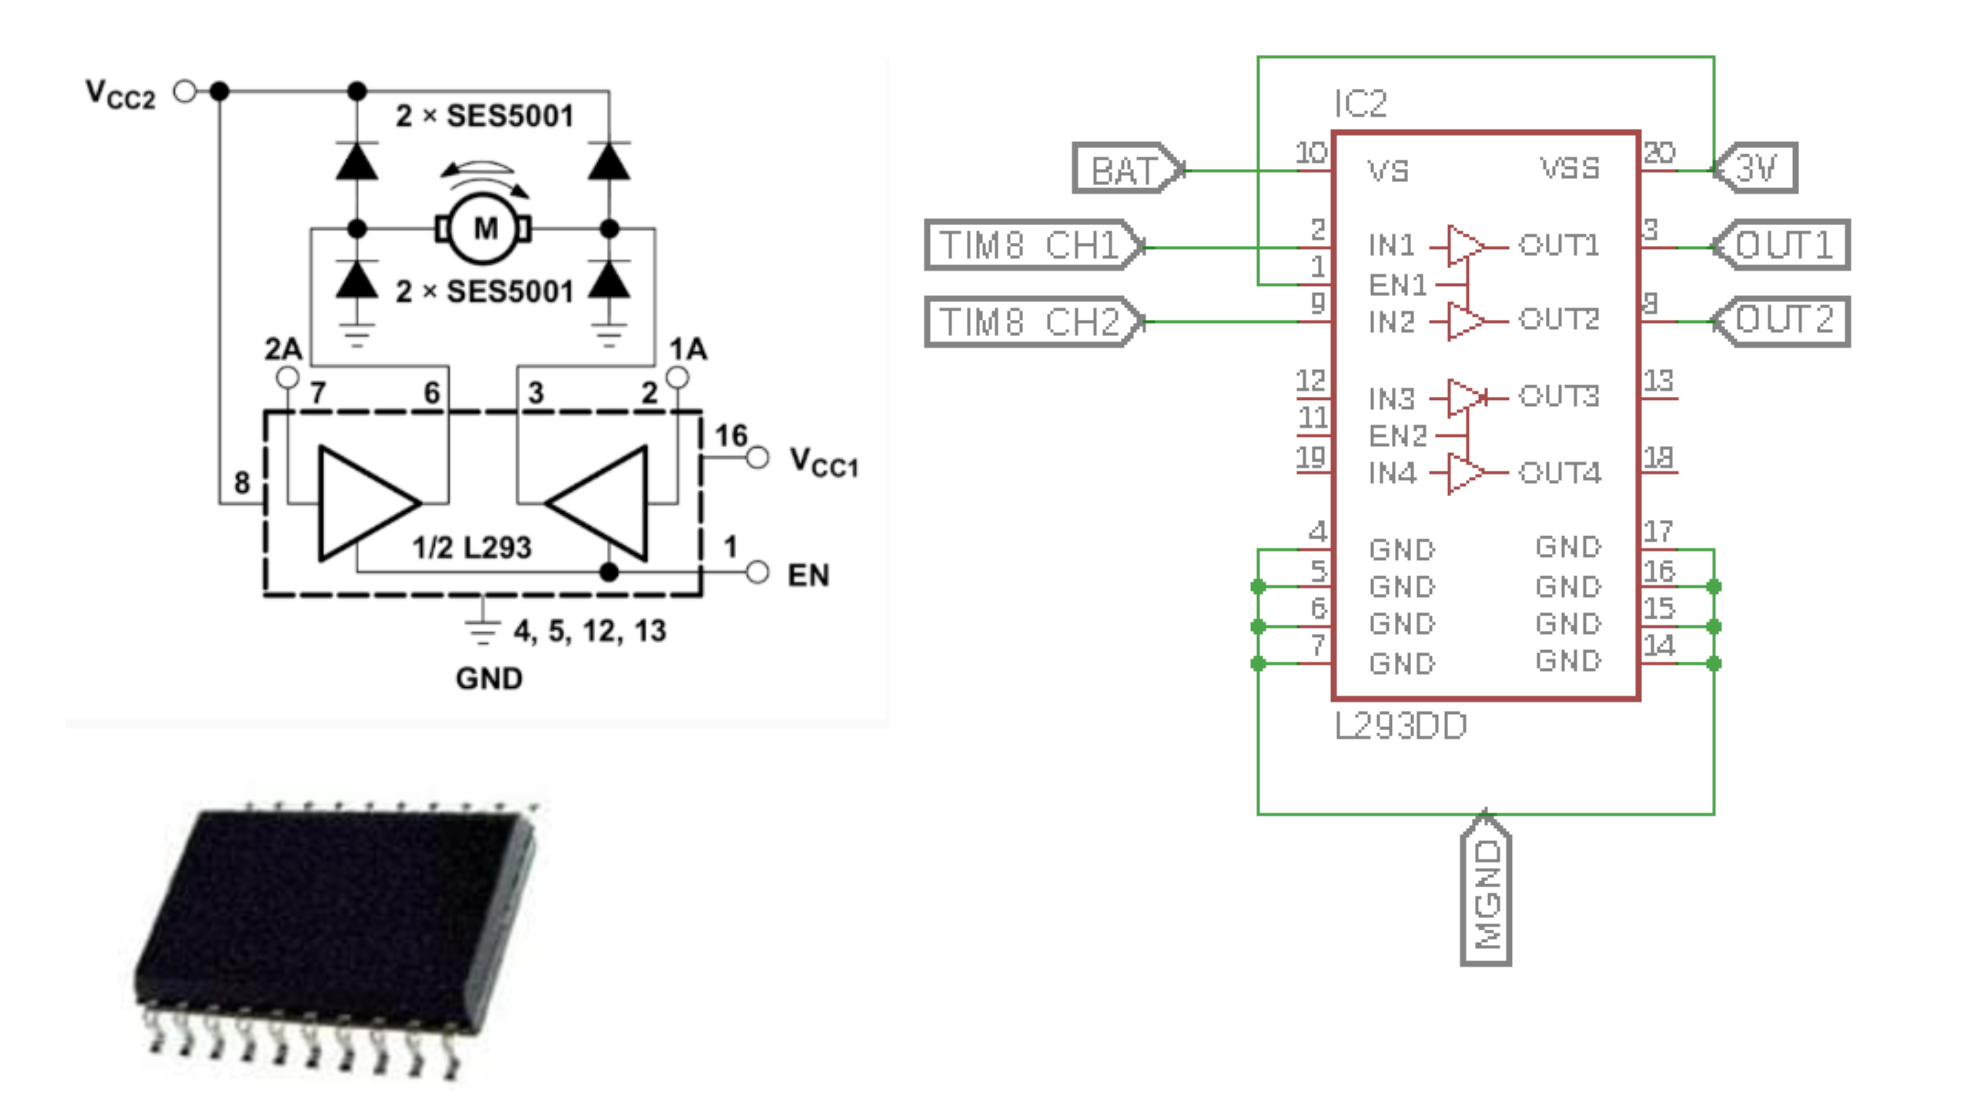
\includegraphics[width=1\textwidth]{./Amir_img/smdHb2.png}
\caption{Bidirectional motor driver L293DDD (H-bridge)}
\end{figure} 
\end{enumerate}
\subsubsection{Voltage regulator}
As shown in bidirectional motor driver schematics, L293DD requires two different voltage level to work properly. Therefore voltage regulator was needed to create the second voltage level required (slightly less than source voltage). The regulator we picked was SMD version of LM2621 which can give out adjustable output in range of 1.2-14 volts. 
 \begin{figure}[H]
\centering
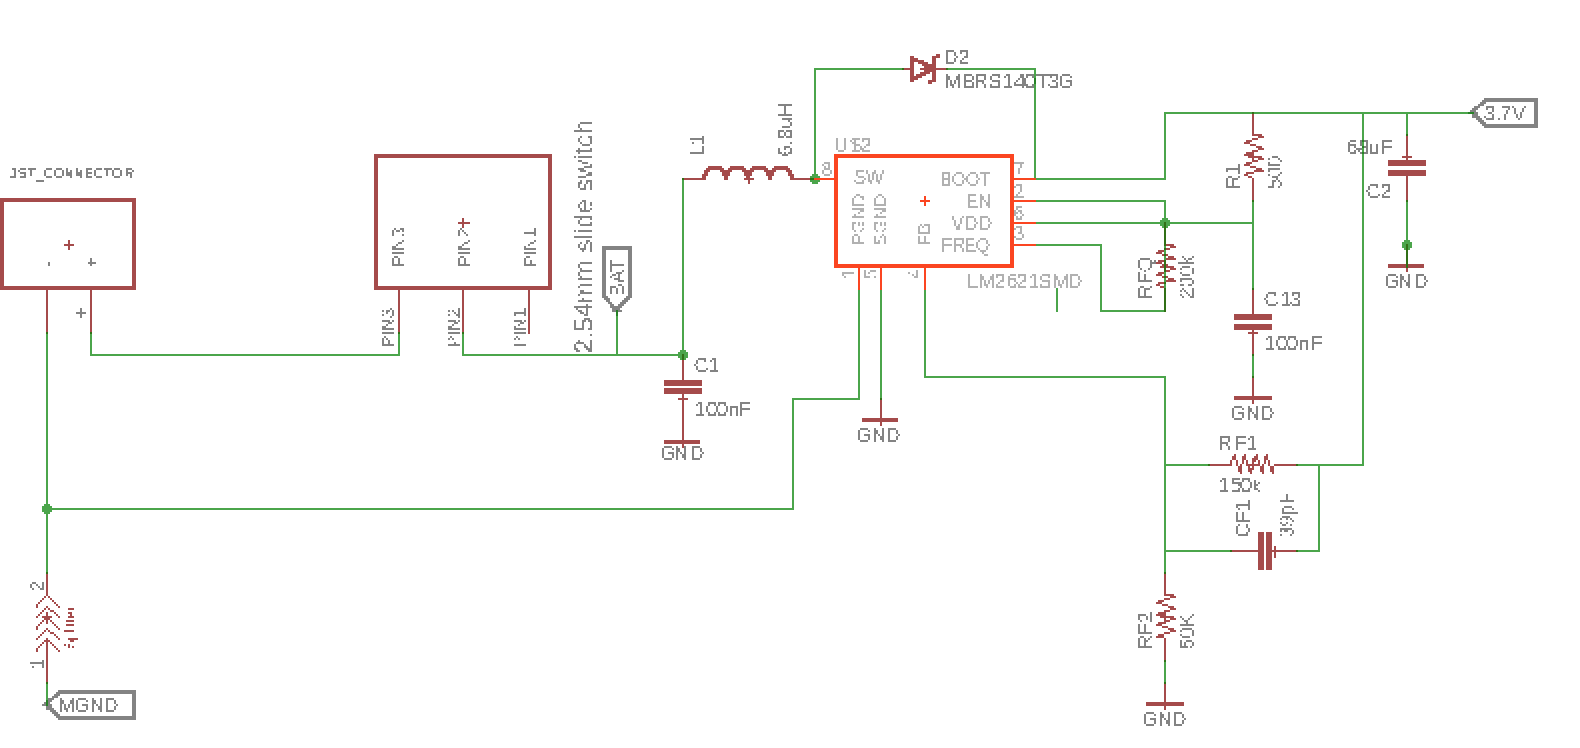
\includegraphics[width=1\textwidth]{./Amir_img/voltageReg.png}
\caption{Voltage regulator in motor controller schematics }
\end{figure} 
\subsubsection{DC Motor and Encoder}
These two components were fully explained in previous section. (Refer to 4.2.1 and 4.2.3)

The remaining components were mostly passive elements such as resistor and capacitors and there were few Schottky diode used for circuit protection purposes. 
\subsection{Crazyflie quad-copter control board}
There were few implementation issues with our separate motor controller circuit. 
\begin{enumerate}
\item Communication issue:
Since the input from user was transmitted to our quad-copter through RF channel, once the connection was setup there was no way to have another connection to our motor driver simultaneously. One way around this issue was to set up another serial communication between motor driver and the MCU of quad-copter. But the delay of the channel could have still been problematic.
\item Too many smd components:
The amount of our controller components along with the hard job of debugging SMD soldering and time consuming process of ordering PCB, given the time window we had, made us to explore more possibilities of implementing more basic controller driver for demonstration purposes.
\end {enumerate}

Studying the schematics of controller board of our quad-copter we realized a lot of components in our design are already considered in in Crazyflie board. Components such as the MCU (STM32 Bit MCU), voltage regulator and ... . We also figured out several GIO pins and analog pins and PWM are left unused on the MCU of our quad-copter. 

\begin{figure}[H]
\centering
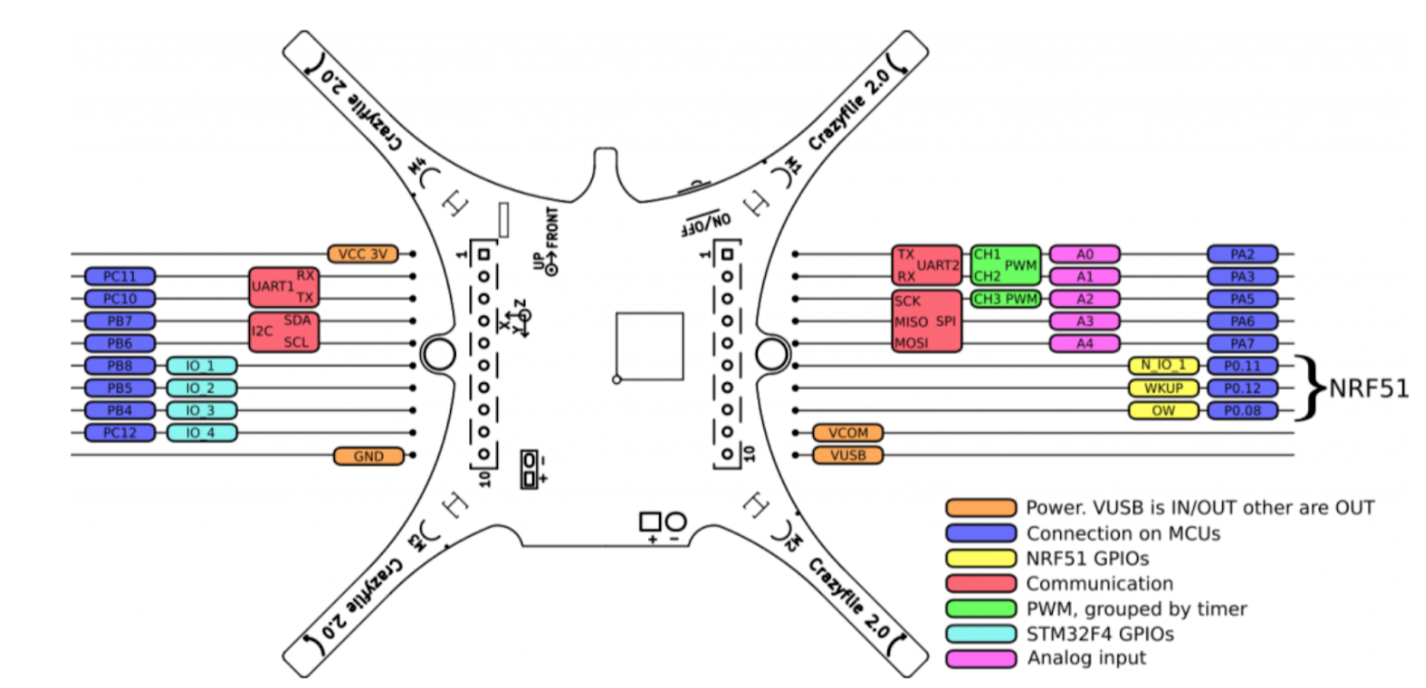
\includegraphics[width=1\textwidth]{./Amir_img/cfPinOut.png}
\caption{Voltage regulator in motor controller schematics }
\end{figure} 

Therefore in order to avoid the redundancy, fully capture the capabilities of our drone and simplify our controller circuit we did not implement the designed PCB.   
Instead we only soldered the needed components on pref board and mounted on top our drone. Again for simplicity we picked the unidirectional motor driver since it had less components and we only had small space of 9 cm x 9 cm grid on our drone. Now that we did not have PCB it was easier to have less components to deal with. 

Some challenges here were how to stabilize and firmly hold the spinning module on top of drone as well as how to power the the motor controller circuit.
As mentioned before, We had already tested powering all 5 motors from our single power source (3.7 V battery), so knowing the fact that this structure would work we added extra parallel connector from battery to motor controller circuit to power the motor of spinning mass and our drone at the same time. 
Also in order to hold the spinning mass module in place we used Styrofoam which was able to hold the module on top of the quad-copter firmly. 
\begin{figure}[H]
\centering
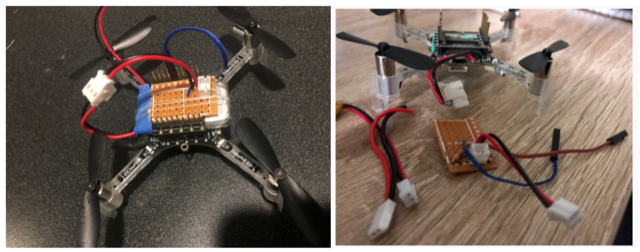
\includegraphics[width=1\textwidth]{./Amir_img/jstConnect.png}
\caption{Parallel jst-connector added to power DC motor of the spinning mass module}
\end{figure} 

\section{System Dynamics}
The ultimate goal of this project was mainly tied to  this part. Where the final outcome was supposed to be a dynamically controllable quad-copter considering the spinning mass module and given all the previously mentioned assumptions. 
\newline Throughout the course of the project this key section turned to be a very complicated control theory problem that even if the right mathematical model approach was given, it would still require a well built hardware and functional accurate software in order to work out. 
In the time frame of 10 weeks we made progress in each of these three main sections, however none became fully completed. As for mathematical derivation and hardware, our approach is already explained. In this part we briefly go over some challenges we faced in software. 
\newline First of all we were not successful in hacking the quad-copter firmware to map user's instant input to our spinning mass module. So next stop we tried to statically upload code to the quad-copter and compare the outcome to expected behavior. As mentioned before one assumption in motor controller circuit was the Crazyflie's MCU is easily programmable so that we we could upload some specific spinning patterns using PWM signals to our system. However it turned out to be much more complicated, than expected, to program the MCU. The code was written in very low level C, which made it hard to understand and very time consuming to upload.
\newline The final flight testing included various unsuccessful attempts where PWM signal was set to high all time and the goal was only to get as close as possible to model a stable flight pattern without making any turns.    
%%%%%%%%%%%%%%%%%%%%%%%%%%%% START OF MOTOR SECTION %%%%%%%%%%%%%%%%%%%%%%%%% 
 
\section{Motor Control and Models}
\subsection{Introduction}
	\subsubsection{Background}
    \indent Due to the constraints of the project design, we are opting to use what motors we have available. These are the same motors that came with the CrazyFlie. \\
Simple specs can be found \href{https://store.bitcraze.io/collections/spare-parts/products/7-mm-dc-motor}{here}.
*Note: no actual spec sheet exists for this component, very little data exists for the component*
Furthermore, in order to create the proper dynamic model for the Spinning Mass Actuator, it was necessary to first develop the DC Motor model and control implementations. Once this was complete, then I could begin finalizing a realistic model. The idea was to work from the ground up adding more and more complexities.
	\subsubsection{Theory}
    \indent The most important aspect of the spinning mass drone project is the motor control. Comparisons between the types of motors we can use (Stepper, servo, DC). Here I present the calculations of a DC motor, the first system modeling is on the motor speed control. The theory is we can determine the speed and the location of the mass using a sinusoidal phase. The second system explores the system modeling with an emphasis on the motor position. A stepper motor with an encoder would allow us both models, but we cannot use one.So we'll begin with a DC motor and no encoder, then improve the design with the implementation of an encoder.
	\subsubsection{Motor Comparisons}
\begin{enumerate}
	\item Permanent Magnet DC Motor
		\\ Great starting torque, good speed regulation. However, torque is limited.
    \item Series DC Motor
		\\ Field is wound with few turns of a large wire carrying full current. Create large starting torque. No speed regulation and prone to damage when run with load. Bad for variable speed drive applications. The speed may vary widely between no load and full load applications. These cannot be used in situations where constant speed is required under varying loads. This problem shouldn't affect us. Also, if run without a load, the speed can increase enough to damage the motor.
    \item Shunt DC Motors
    	\\ Great speed regulation due to shunt field can be excited separate from current windings (due to parallel connections).
    \item Compound DC Motors
    	\\ Separately excited shunt field. Good starting torque but prone to control problems during variable speed drive applications. This motor has better torque and speed regulations than a shunt.
    \item Stepper Motor
    	\\ Come in a wide range of angular resolution. Steppers don't require encoders, can accurately move between their poles. Open loop (without encoder), close loop (with encoder). A single rotation requires more current exchanges through the windings. Torque degradation at higher speeds is observed. Traditional Stepper motors operate in an open loop constant current mode. Due to this design, energy is conserved due to the lack of an encoder. However, due to this operation, a significant amount of heat is created. With the addition of an encoder, can be controlled with a closed loop model. Excellent for speeds less than 2,000 RPM and for low to medium acceleration rates and hight holding torque. 
    \item Servo Motor
    	\\ Requires an encoder to keep track of their position. Using the encoder, servos can measure the difference between the motor encoder and the commanded position (closed loop). Supplies the motor with the current required to move or hold the hold. Excellent for situations requiring speeds greater than 2,000 RPM and for high torque at high speeds. 
    
\end{enumerate}
\subsection{Physical Representations}
	\subsubsection{Schematics}
\begin{figure}[ht]
\centering
\shadowbox{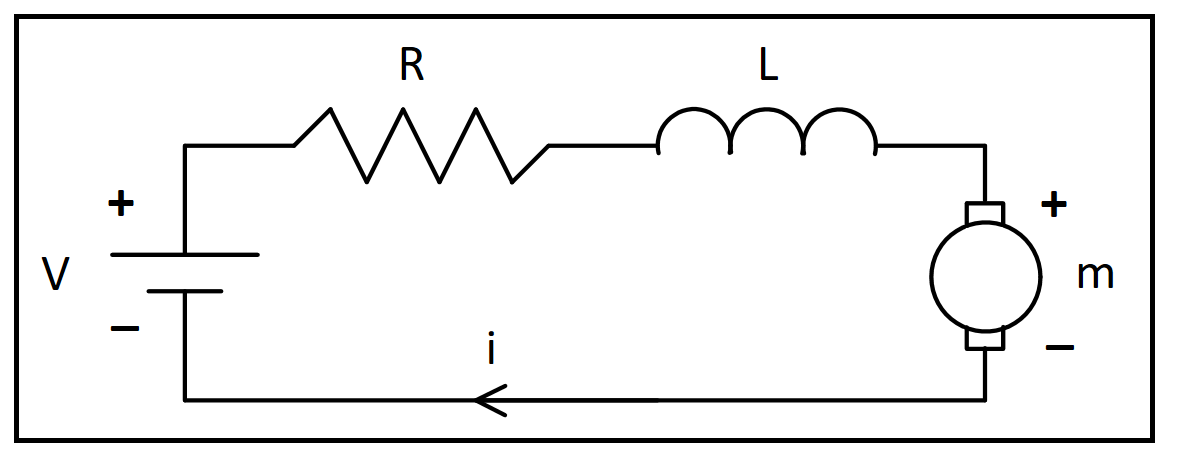
\includegraphics[width = 0.6\textwidth]{./Angel_img/DC_MOTOR_CIRCUIT.png}}
\caption{\label{fig:dc1}DC motor schematics}
\end{figure}

\break
\begin{figure}[ht]
\centering
\shadowbox{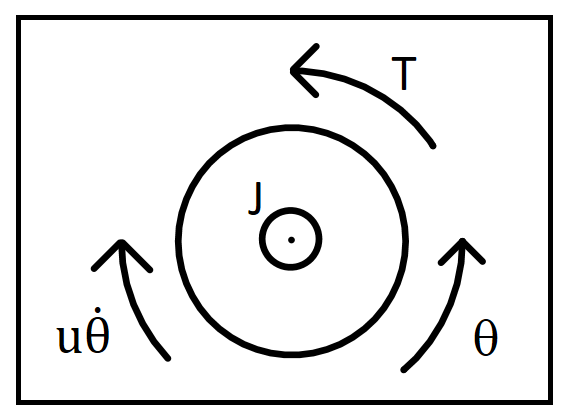
\includegraphics[width = 0.4\textwidth]{./Angel_img/DC_MOTOR_ROTOR.png}}
\caption{\label{fig:dc2}DC motor rotor forces}
\end{figure}

	\subsubsection{Assumptions}
    The assumptions made are relatively the same for both models. We assume that the input of the system will be the voltage source (V). In the speed control model, we assume the output is the rotational speed of the rotor shaft ($\dot{\theta}$), depicted in Figure \ref{fig:dc2}. All components are rigid. The friction torque is proportional to the rotor angular velocity. We assume the magnetic field permeated is constant. Similarly for the Position model, the assumption of the about now includes the rotational displacement as one of the outputs.
	\subsubsection{Parameters and Components}
    \begin{tabular}{cccc}
\textbf{Symbol}		& \textbf{Name}			& \textbf{Data}			& \textbf{Units} \\
V 				& Voltage Source			& 3.7v lipo battery & V	\\
R 				& Resistor					& 10 		 & $\Omega $		\\
L 				& Inductor					& 1 				 & H	\\
m 				& DC Motor					& 7mm brushed		 & -	\\
i 				& Electric Current			& -				 & A	\\
T 				& Motor Torque				& -				 & [$N \cdot m$]	\\
J				& Rotor Moment of Inertia 	& 0.1 & $[kg \cdot m^{2}]$  	\\
$ \theta $		& Angular Displacement 		& -  & 	rad\\
$ \dot{\theta}$ & Angular Velocity 			& -  & [$ \frac{rad}{sec}	$]\\
u 				& Friction Coefficient		& 0.1  		& $[N \cdot m \cdot s]$	\\
$ K_{i} $ 		& Motor Constant Coefficient& 0.1  & [$ \frac{N \cdot m}{A}$]	\\
$ E_{b}	$		& Motor back EMF			&	- & [$ \frac{N \cdot m}{A}$]\\
\end{tabular}
\subsection{Speed Control Derivations}
	\subsubsection{Speed Equations}
    The torque generated by a DC motor is proportional to the current and the magnetic field strength. For simplicity we assume the magnetic field is constant. This further simplifies our model by making the torque proportional only to the current. The torque equation is

\begin{equation}
 T = K_{i} \psi i
\end{equation}

\noindent where $ \psi $, is the flux, and the $ K_{i} $ is a constant factor. Because of our constant field assumption, this equation becomes 

\begin{equation}
T = K_{i} i
\end{equation}


\noindent The back emf (Electromotive Force) is governed by the following equation

\begin{equation}
m = E_b = K_{i} \dot{\theta}
\end{equation}

*** Note: The Constant Coefficients aren't necessarily the same, but due to our assumptions and their SI units, we can consider them equal. ***
\break

\noindent Looking at Figure \ref{fig:dc1}, we can apply Kirchoff's Voltage Law to derive the following system relationship

\begin{equation}
L \frac{di}{dt} + Ri + K_{i} \dot{\theta} = V
\end{equation}

\noindent Applying Newton's Second Law on Figure \ref{fig:dc2} we derive the following equation

\begin{equation}
J \ddot{\theta} + u \dot{\theta} = K_{i} i
\end{equation}

Applying the Laplace Transform to equations (4) and (5) we obtain

\begin{equation}
LI(s)s + RI(s) + K_{i} \Theta(s)s = V(s)
\end{equation}

\begin{equation}
J \Theta (s) s^{2} + u \Theta (s) s = K_{i}I(s)
\end{equation}

We want to consider the Voltage as our only input thus we solve using I(s) and arrive at the Open Loop Transfer Function. 

\begin{equation}
\frac{s \Theta(s)}{V(s)}  = \frac{K_{i}}{JLs^{2} + JRs +uLs + uR + K_{i}^{2}}
\end{equation}

\noindent which can be simplified into this form

\begin{equation}
H(s) = \frac{\dot{\Theta(s)}}{V(s)}  = \frac{K_{i}}{(Js+u)(Ls+R) + K_{i}^{2}}  \hspace{1cm} [\frac{rad}{V \cdot sec}]
\end{equation}

Now, we can derive our state space equations.
From the transfer function we can form our state space representation of the system

\begin{equation}
\frac{d}{dt} \begin{bmatrix} \dot{\theta} \\ i \end{bmatrix} = \begin{bmatrix} - \frac{u}{J} & \frac{K_{i}}{J} \\ - \frac{K_{i}}{L} & - \frac{R}{L}  \end{bmatrix} \begin{bmatrix} \dot{\theta} \\ i \end{bmatrix} + \begin{bmatrix} 0 \\ L^{-1} \end{bmatrix} V
\end{equation}
and
\begin{equation}
z = \begin{bmatrix} 0 & 1 \end{bmatrix} \begin{bmatrix} \dot{\theta} \\ i \end{bmatrix}
\end{equation}

   	\subsubsection{Speed MATLAB}
    *** Note: MATLAB 2017b can sometimes crash or take a long time to compile when using the syms function, especially with a lot of variables. ***
We use MATLAB for our purposes of simulation due to the comprehensive tools and applets provided by the software for the purpose of simulation. Python is a great alternative, however, there is greater documentation available for MATLAB.
\begin{figure}[H]
\centering
\shadowbox{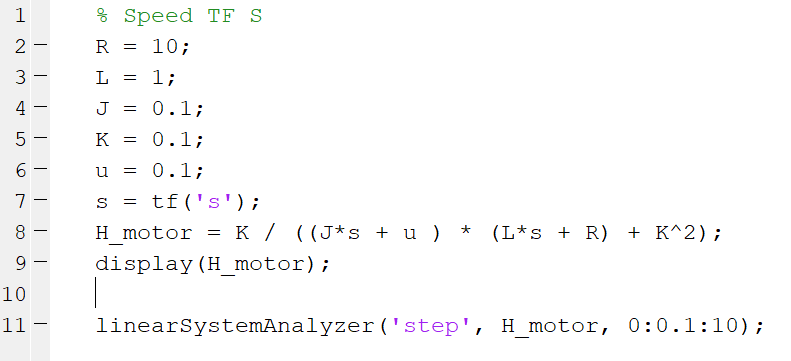
\includegraphics[width = 0.7\textwidth]{./Angel_img/DC_SPEED_1.png}}
\caption{\label{fig:code_speed1} This is the code snippet for the transfer function in matlab}
\end{figure}

\begin{flushleft}
\noindent The output for the code in Figure \ref{fig:code_speed1} should look like this 
\end{flushleft}
\fbox {
    \parbox{\linewidth}{
	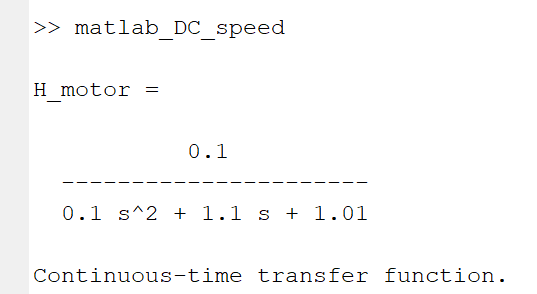
\includegraphics[width = 0.4\textwidth]{./Angel_img/DC_SPEED_2.png}
    }
}
\break
\noindent A box should appear after a loading bar sequence finishes. The results appear as follows

\begin{figure}[H]
\centering
\shadowbox{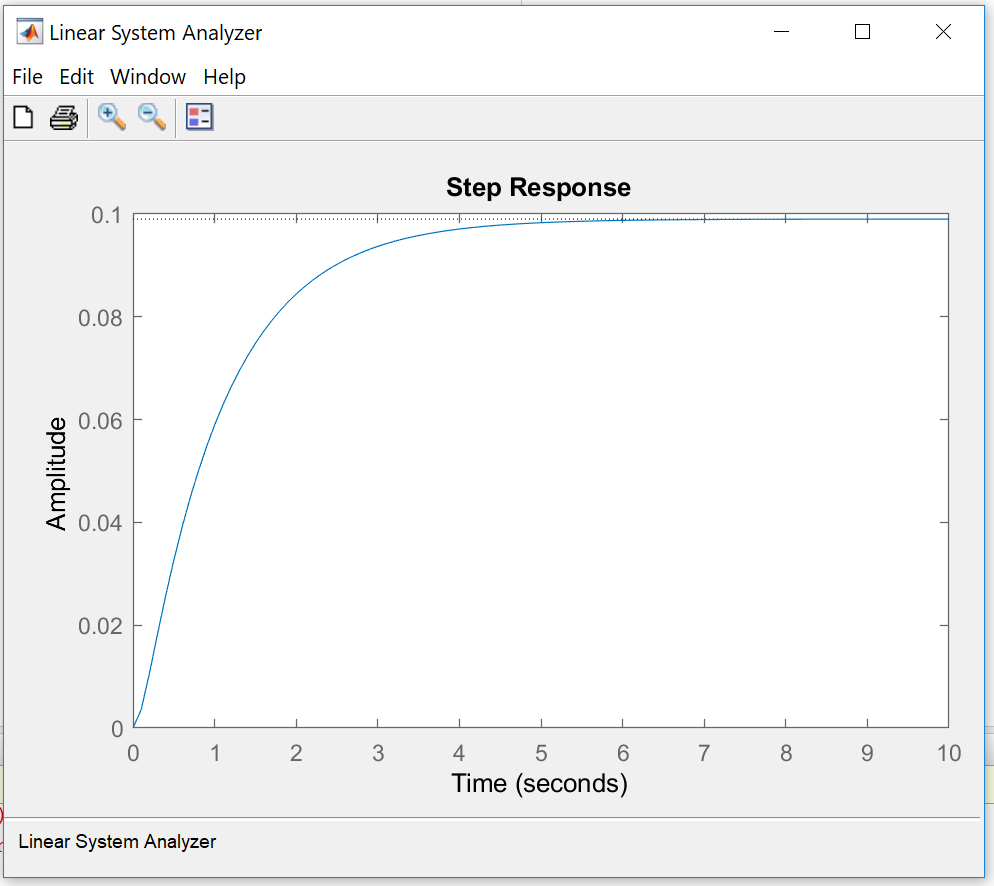
\includegraphics[width = 0.7\textwidth]{./Angel_img/DC_SPEED_LSA.png}}
\caption{\label{fig:code_speedLSA} This is the result of the Linear System Analyzer function}
\end{figure}
	\subsubsection{Speed Simulink}
    We will model the system analyzing the forces and torques on the DC motor rotor. To begin you have to model the integrals of our current and displacement. We can derive these models from the equations we formulated earlier. The models for equations (6) and (7) are

\begin{figure}[H]
\centering
\shadowbox{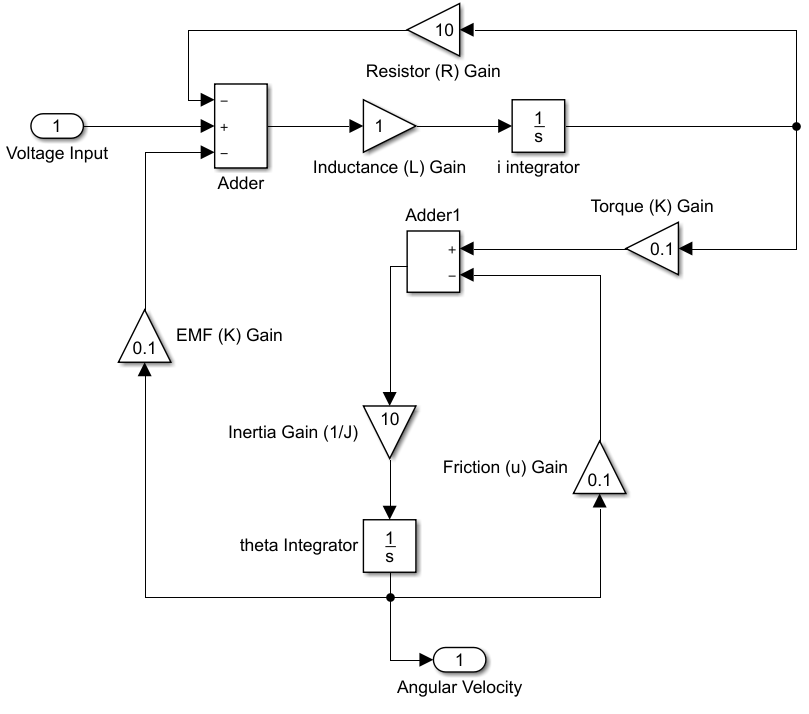
\includegraphics[width = 0.8\textwidth]{./Angel_img/DC_SPEED_SIMU.png}}
\caption{\label{fig:code_speed_simu} Simulink representation of the DC Motor model}
\end{figure}

To run any form of simulation, you have to modify the input and output signals of the model. We do this by right clicking the line between the input and the model then selecting "Linear Analysis Points" and selecting "Open Loop Input" for the input and "Open Loop Output" for the output
\begin{figure}[H]
\centering
\shadowbox{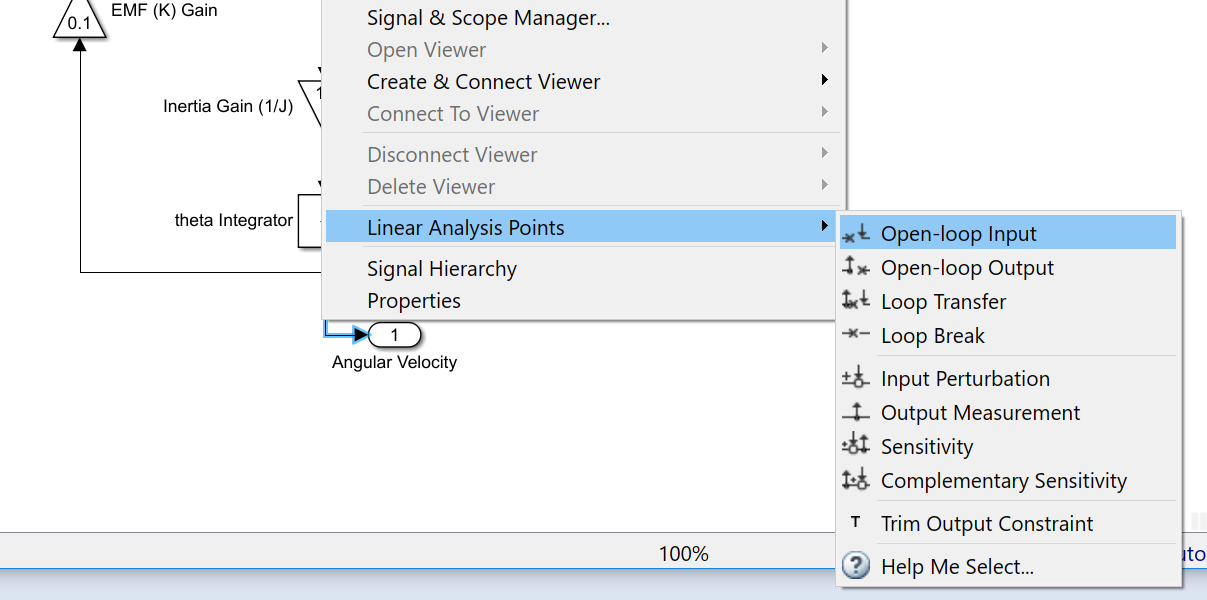
\includegraphics[width = 0.6\textwidth]{./Angel_img/DC_SPEED_SIMU1.png}}
\caption{\label{fig:code_speed2} necessary adjustments to the signals}
\end{figure}

\noindent We have to ensure our Simulink (Figure \ref{fig:code_speed_simu}) model matches up with our mathematical model we derived earlier (equations (6) and (7)). We have already performed the first part of this process and that was plotting the Linear System Analysis in response to a step function. Next, in the Simulink project, we click on Analysis on the top and proceed to Linear Analysis. This prompts the Linear Analysis Tool, in the top right, we select the "Step" plot. We should see this 

\begin{figure}[H]
\centering
\shadowbox{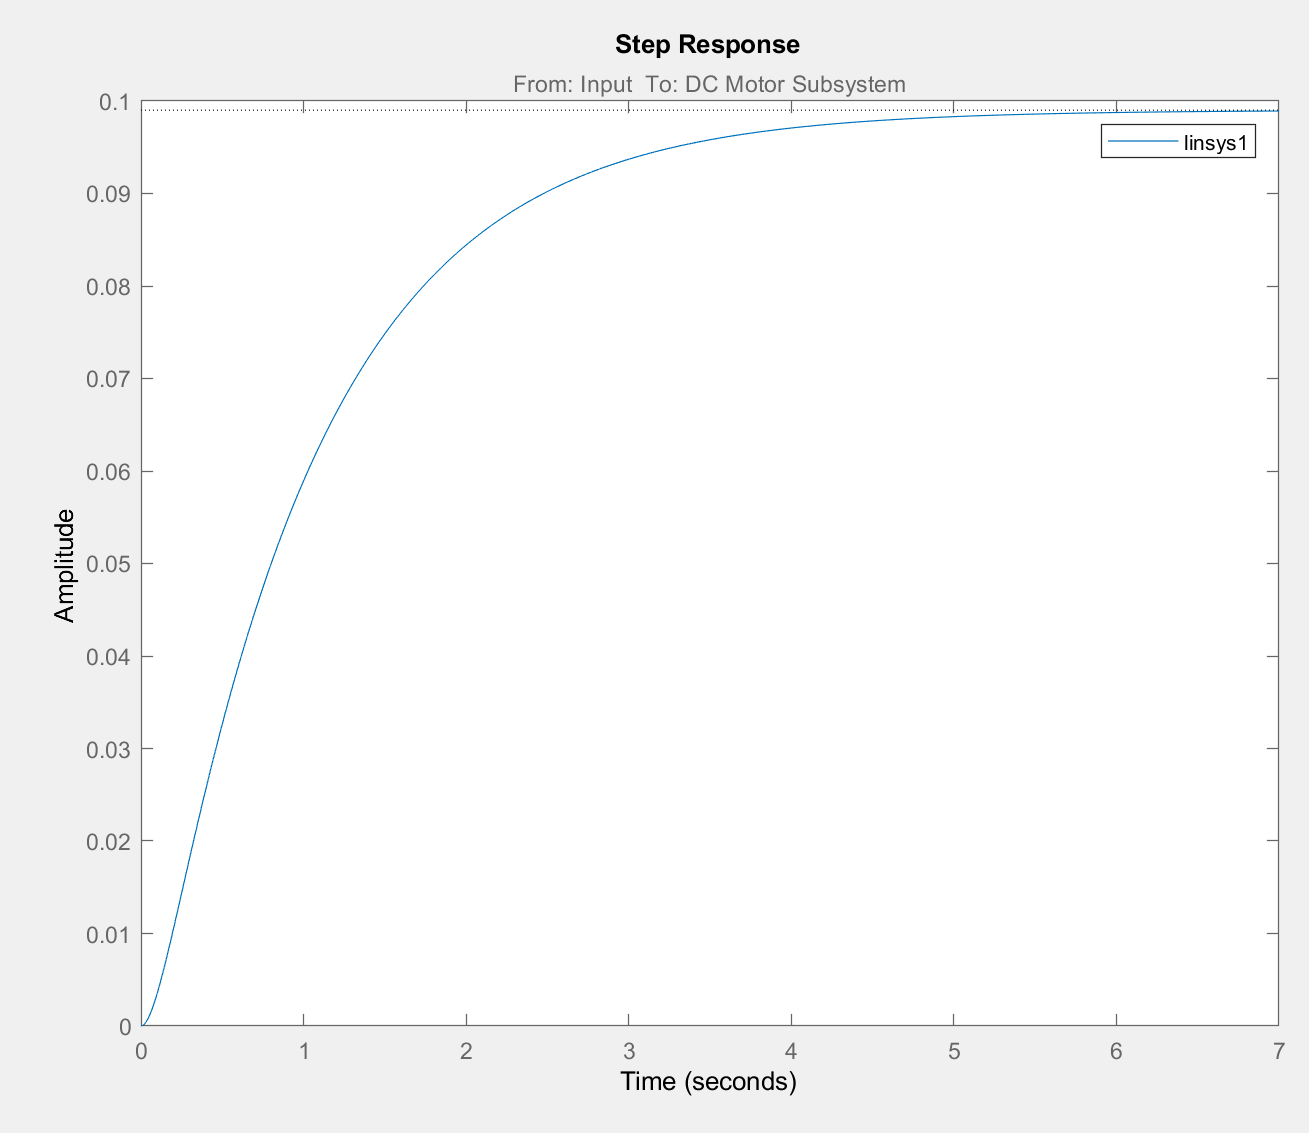
\includegraphics[width = 0.5\textwidth]{./Angel_img/DC_SPEED_SR.png}}
\caption{\label{fig:SPEED_SIMU} Linear Analysis Tool, system response to a step input}
\end{figure}

\noindent Comparing Figure \ref{fig:SPEED_SIMU} with Figure \ref{fig:code_speedLSA} we can see that the mathematical model step response matches the Simulink model step response. This confirms our models are accurate.
    \subsubsection{PID Design}
    
\begin{figure}[H]
\centering
\shadowbox{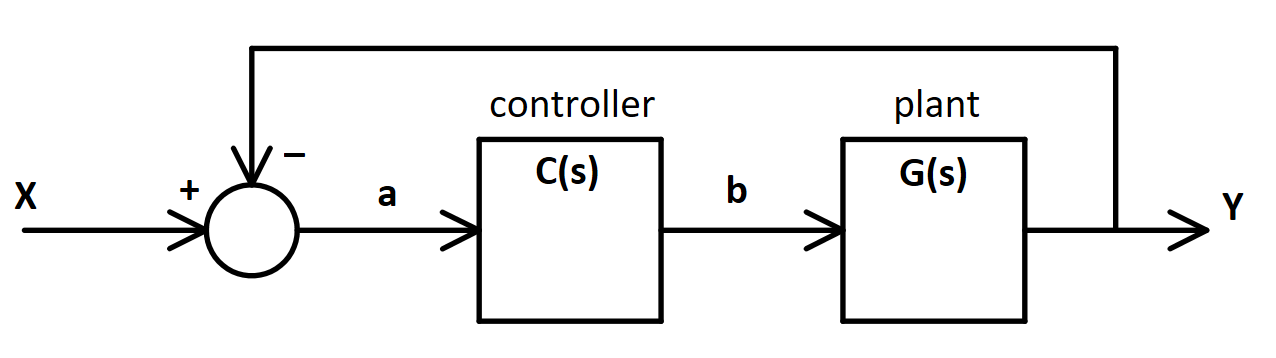
\includegraphics[width = 0.5\textwidth]{./Angel_img/DC_SPEED_PID.png}}
\caption{\label{fig:SPEED_PID} Control System Model}
\end{figure}

\noindent The structure of the Control system in Figure \ref{fig:SPEED_PID} is based on our derived mathematical equations. A PID is a three term controller, it is continuously calculating an error value (in our case a) as the difference between our desired value and the measured value.The three terms are a proportional term, an integral term and a derivative term. Together we get the equation 

\begin{equation}
c(t) = K_{p}a(t) + K_{i}\int ^{t}_{0} a(\tau) d\tau + K_{d} \frac{da(t)}{dt}
\end{equation}

The Transfer Function form is 

\begin{equation}
C(s) = K_{p} + \frac{K_{i}}{s}+K_{d} s
\end{equation}

\noindent Where $K_{p}$, $K_{i}$, and $K_{d}$ are constant coefficients of the controller. *** NOTE: $K_{i}$ is not to be confused with the $K_{i}$ from our mathematical derivations. ***

\noindent the values for your PID controller coefficients are largely dependent on the values you set for your parameters. Variations exist, and tuning is necessary for an optimal controller. 

\begin{figure}[H]
\centering
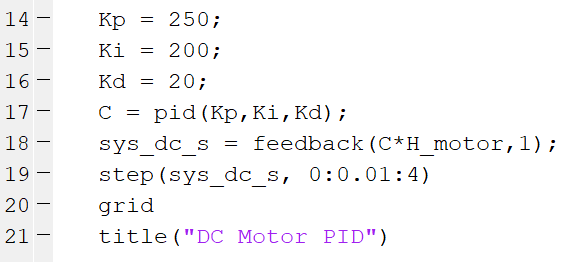
\includegraphics[width = 0.5\textwidth]{./Angel_img/DC_SPEED_PIDCode.png}
\caption{\label{fig:code_speed_PIDCode} This is the code snippet for the PID controller in matlab}
\end{figure}

After tuning my values, I found $K_{p} = 250$, $K_{i} = 200$, and $K_{d} = 20$ where fairly good. An analysis if they're reasonable will have to be performed later. The Figure below demonstrates what the graph looks like after before and after tuning.

\begin{figure}[H]
\centering
\shadowbox{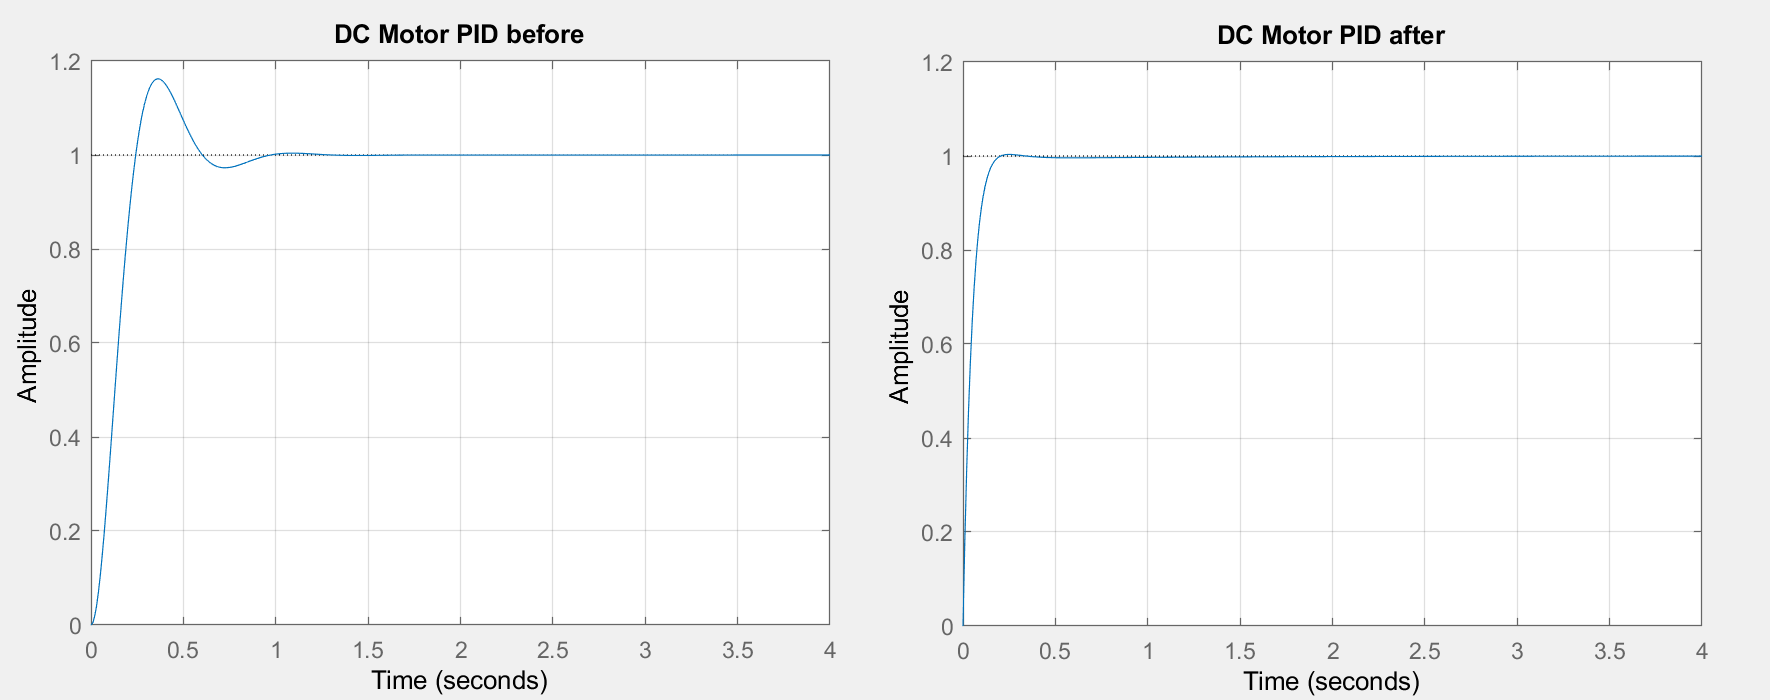
\includegraphics[width = 1\textwidth]{./Angel_img/DC_SPEED_PIDtune.png}}
\caption{\label{fig:code_speed_PIDtune} This is the code snippet for the PID controller in matlab}
\end{figure}
\subsection{Position Control Derivations}
	\subsubsection{Position Equations}
    The position equations are almost identical to the speed equations we derived before. The prominent change in this model is our assumption of the output variable, it is now our angular displacement. This directly affects out state space estimation equation and our transfer function.

Applying the Laplace Transform to the equations we obtain

\begin{equation}
LI(s)s + RI(s) + K_{i} \Theta(s)s = V(s)
\end{equation}

\begin{equation}
J \Theta (s) s^{2} + u \Theta (s) s = K_{i}I(s)
\end{equation}

We want to consider the Voltage as our only input thus we solve using I(s) and arrive at the Open Loop Transfer Function. 

\begin{equation}
\frac{\Theta(s)}{V(s)}  = \frac{K_{i}}{s(JLs^{2} + JRs +uLs + uR + K_{i}^{2})}
\end{equation}

\noindent which can be simplified into this form

\begin{equation}
H(s) = \frac{\Theta(s)}{V(s)}  = \frac{K_{i}}{s((Js+u)(Ls+R) + K_{i}^{2})}  \hspace{1cm} [\frac{rad}{V}]
\end{equation}

Now, we can derive our state space equations.
From the transfer function we can form our state space representation of the system

\begin{equation}
\frac{d}{dt} \begin{bmatrix} \theta \\ \dot{\theta} \\ i \end{bmatrix} = \begin{bmatrix} 0 & 1 & 0\\ 0 &- \frac{u}{J} & \frac{K_{i}}{J} \\ 0 & - \frac{K_{i}}{L} & - \frac{R}{L}  \end{bmatrix} 
 \begin{bmatrix} \theta \\ \dot{\theta} \\ i \end{bmatrix} + \begin{bmatrix} 0 \\ 0 \\ L^{-1} \end{bmatrix} V
\end{equation}
and
\begin{equation}
z = \begin{bmatrix} 1 & 0 & 0 \end{bmatrix} \begin{bmatrix} \theta \\ \dot{\theta} \\ i \end{bmatrix}
\end{equation}

   	\subsubsection{Position MATLAB}
    
   \begin{figure}[H]
\centering
\shadowbox{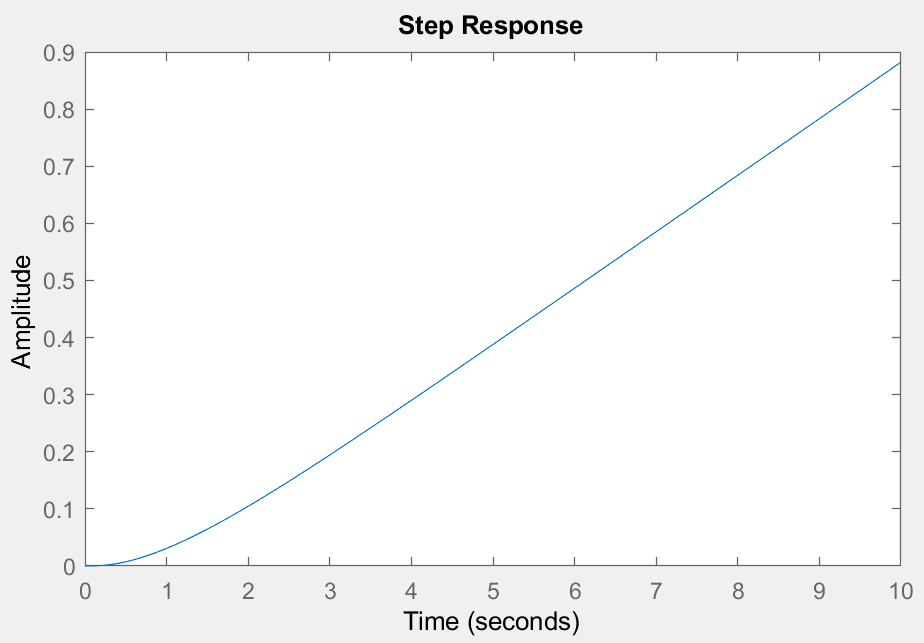
\includegraphics[width = 0.7\textwidth]{./Angel_img/POSITION_MATLAB_1.png}}
\caption{\label{fig:position_1} Transfer Function response to the Linear System Analysis function}
\end{figure}

   \begin{figure}[H]
\centering
\shadowbox{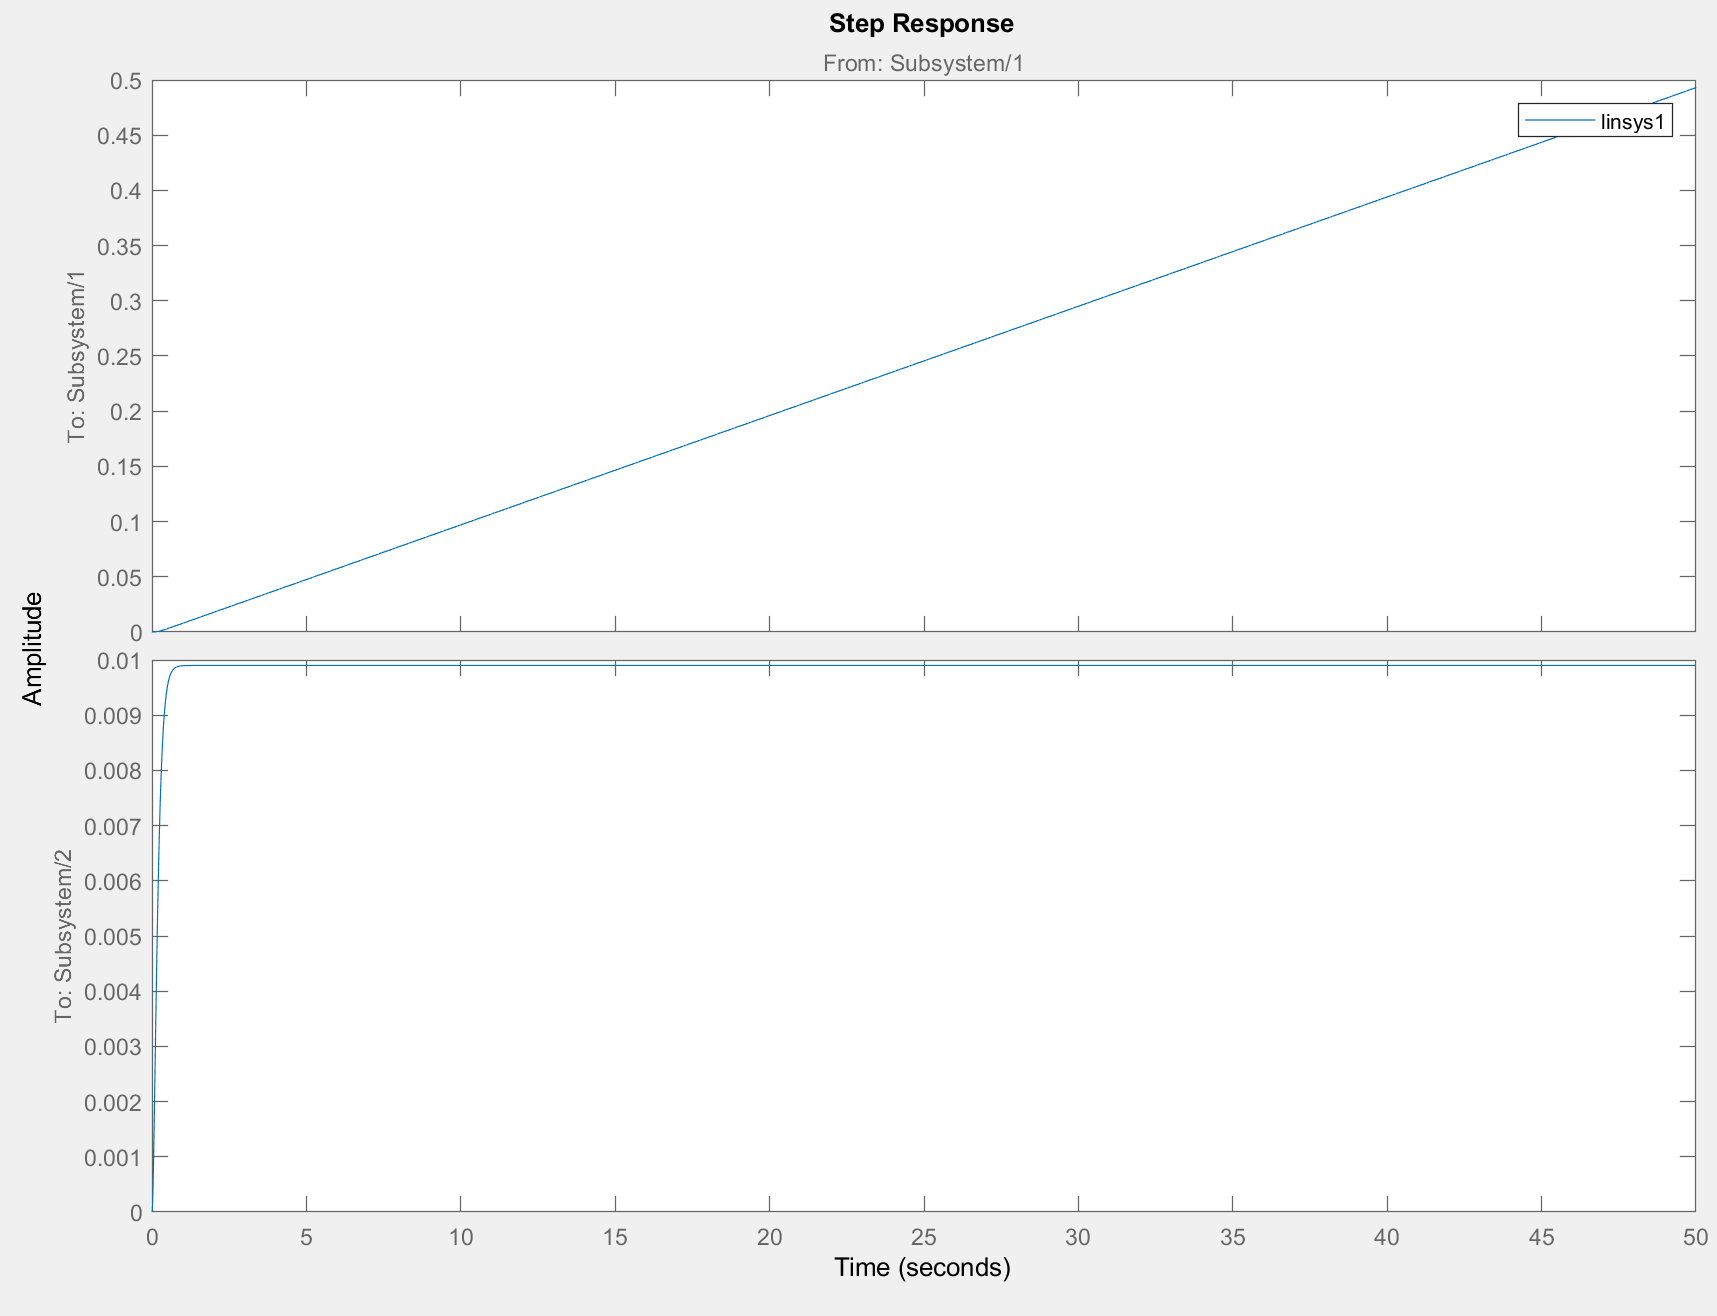
\includegraphics[width = 0.7\textwidth]{./Angel_img/POSITION_MATLAB_2.png}}
\caption{\label{fig:position_2} Simulink Model Analysis using the Linear Analysis Tool}
\end{figure}

The graph in Figure \ref{fig:position_1} matches the upper graph in Figure \ref{fig:position_2} thus the simulink model matches the mathematical simulation model.

	\subsubsection{Position Simulink}
    
    This (Figure \ref{fig:position_3}) is largely similar to the position Simulink model, the difference being the output is now an angular displacement. Meaning, our original output goes through an integrator block. 
\begin{figure}[H]
\centering
\shadowbox{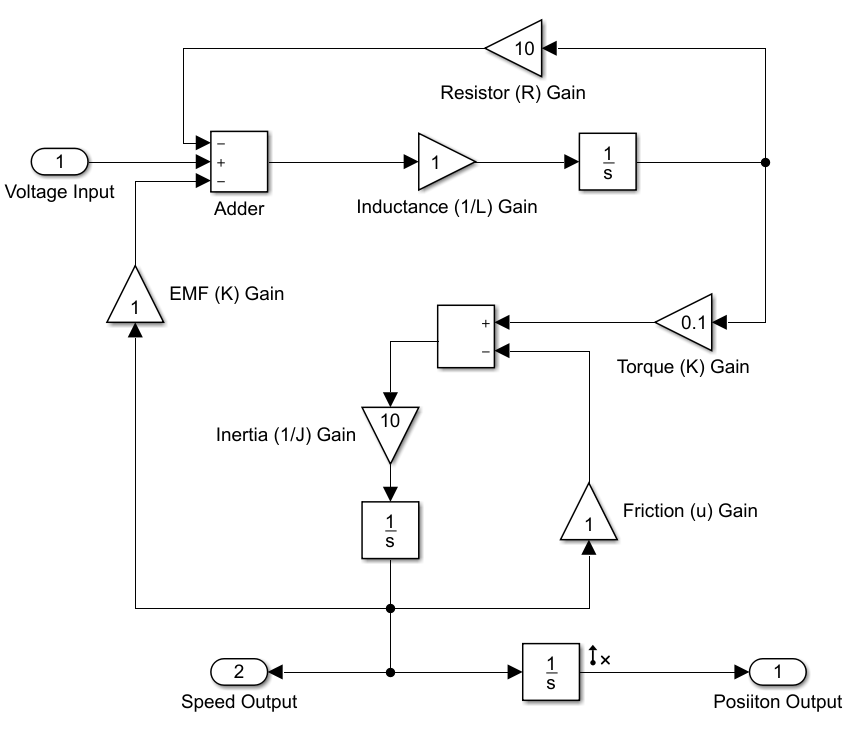
\includegraphics[width = 0.7\textwidth]{./Angel_img/POSITION_MATLAB_3.png}}
\caption{\label{fig:position_3} Simulink Model Analysis using the Linear Analysis Tool}
\end{figure}
    
    
 \subsection{PID Design}
 This process is similar to our previous PID implementation. 
 \begin{equation}
c(t) = K_{p}a(t) + K_{i}\int ^{t}_{0} a(\tau) d\tau + K_{d} \frac{da(t)}{dt}
\end{equation}

The Transfer Function form is 

\begin{equation}
C(s) = K_{p} + \frac{K_{i}}{s}+K_{d} s
\end{equation}

\noindent Where $K_{p}$, $K_{i}$, and $K_{d}$ are constant coefficients of the controller. *** NOTE: $K_{i}$ is not to be confused with the $K_{i}$ from our mathematical derivations. ***

\noindent the values for your PID controller coefficients are largely dependent on the values you set for your parameters. Variations exist, and tuning is necessary for an optimal controller. 

\subsection{Dynamic Model}
This section of the research is largely incomplete. The intention was to work from the ground up, beginning this portion after having completed the Motor modeling. Due to time constraints we could not finish this.
\subsubsection{Physical Representation}

\begin{figure}[H]
\centering
\shadowbox{\includegraphics[width = 0.5\textwidth]{./Angel_img/DYNAMIC_BIRD.png}}
\caption{\label{fig:dynamic_birdseye} unfinished Top View of OCSM Dynamic Model}
\end{figure}

\begin{figure}[H]
\centering
\shadowbox{\includegraphics[width = 0.5\textwidth]{./Angel_img/DYNAMIC_SIDE.png}}
\caption{\label{fig:dynamic_side} unfinished Side View of OCSM Dynamic Model}
\end{figure}

From Figure {\ref{fig:dynamic_side}} we can derive the following equations of inertia. I feel that it is crucial in the representation of the model that this be as correct as possible. Thus my assumptions do not exclude the mass of the rod. Also, I felt it was necessary to use the Parallel Axis Theorem.

\begin{equation}
 I = \frac{1}{3}M_{rod}L^{2}+\frac{2}{5}M_{sphere}R^{2}+M_{sphere}(L+R)^{2}
\end{equation}
\subsection{3D Simulation}
The 3D simulation demonstrates the control of both the position and speed. The model can be seen in 

\begin{figure}[H]
\centering
\shadowbox{\includegraphics[width = 0.5\textwidth]{./Angel_img/POSITION_MATLAB_4.png}}
\caption{\label{fig:position_4} 3D model of the motor and OCSM module}
\end{figure}
\vspace{5cm}


%% =======================================
%% WORK ON THIS GUYS
%% =======================================
\section{Results}
Using Newton's fundamental law of physics, we are able to derive systems of equations that characterize the dynamics of our system. However, due to the complexity introduced by rotational acceleration, even in quaternion, no close-solution in the form of $\dot{s} = f(s)$ is analytically derived. Moreover, solving the equations in the form $f(\dot{s},s)$ numerically in Matlab yields no solutions. \par
%  LIN :done
As the exact Mathematical model we derived yields no fruitful results, we turned to building a simulation environment using Matlab's toolbox, in the hope that we can get an idea of our system dynamics in the simulation. \par
We have built a decent 3D model for the quandcopter and then we have generated several dynamic 3D simulation. Due to the limitation of our current math model, we had to make assumptions that the thrust force is always applied perfectly at the center of the core of the quadcopter and the quadcopter can only pitch inside a single plane. Theoretically, that could be possible if we have a perfectly assembled quadcopter and perfect controlling motor. Under these assumptions that we have ideal hardware and software, the simulation does a pretty good job.\par
We have obtained three major insights and parameters from the simulation. First,the spinning rate should be closer to about 10 rounds per second, otherwise it will easily get flipped over. Due to the assumptions we made, the accuracy of this value would be low. Second, the pitching angle for the movement should be around 22 degree for our quadcopter otherwise it won't move efficiently. This value is much more reliable because our assumption doesn't directly decrease this parameter's accuracy since the pitching direction is inside the same plane with the movement direction vector. Finally, the thrust force should be about 1.2 times bigger than the gravitational force of our quadcopter. This parameter is also very reliable since the thrust force is also inside the same plane with the movement direction vector and it's confirmed to be pretty accurate when we did the real world tests.\par
%  Angel PLS SUMMARISE RESULTS HERE.
Results of the motor analysis are conclusive. As shown by the data collected from the linear analysis function in matlab and the Simlink linear anaylsis tool, the models are a perfect match. This is good because this is our base case model. Given the total drone derived model. If we were to simplify heavily, we could ultimately result in this DC motor model. We still need empirical data on the various types of motors available. We could not procure all the motors or tests we needed to perform due to the time and budget constraints. Lastly, the incomplete mathematical model meant we would have to do real time experiments with the motors in order to understand the behavior.
% Amir PLS SUMMARISE IMPLEMENTATION RESULTS HERE.
With the support of our theoretical results, we started designing our spinning mass module, followed by implementing motor driver circuit and hacking the crazyflie.
 The final outcome was supposed to be a dynamically controllable quad-copter however we modified the final prototype as we were not able to obtain a functional math model for full implementation of we started with. Also our hardware and software issues limited the scope of our project for the short given period of time.
 \newline
 Other issue to be addressed here, was our planning task. By getting to this part of the project,
 we realized due to some bad assumptions we made the path of our progress got deviated few times during past ten weeks. This could be meanly due to having wrong priorities. For example at the very beginning we started by setting up the joystick controller for our drone without considering whether we could map the user's input to our mass module in the time frame given, which turned out to be very hard and we could not complete it. Or for instance we stared configuring our rotary encoder before testing our spinning mass module on the quad-copter. Again with the wrong priority order, we spent time on secondary goals while our primary targets were way further to accomplished. We also learned about the design process of projects in this scope. The fact that your given problem is not always nice and smooth linear system with straightforward solution. We thought we should wait to finish the theoretical modeling first then move to building the module. While having a mathematical model is definitely necessary for such problems, on site testing in last two weeks showed us sometimes it is better to take reverse engineering approach. Visualizing
 the natural behavior of the system can bring us some useful insights that are not quite obvious or even reachable through theoretical equation deriving. Had we had another chance to start this project we would have started working on physical modeling from first few weeks as we realized theoretical modeling and actual implementation would work better if applied in parallel way. 
 \newline
 Finally working on this project brought us some of very fundamental concepts, that we had learned before but this time facing them in an interesting unique way. Newton's third law, for instance, was not something new. However the understanding of how to apply it for a flying vehicle and its important to derive the mathematical equations of such system was like learning something new from scratch. Similarly, we had heard multiple times about pull down resistor in different classes but it was in this project that due to logic error in our initial motor circuit we learned again about pull down resistor. This time however we added it to our circuit and fully saw the results of adding such resistor in the behavior of our circuit. This aspect of our project can be considered as our interesting challenges where most of our learnings from this project happened. The part that was motivating and drove us forward.      
 
\section{Further Work}  
A few simple special cases can be used to test the validity of the Mathematical model. Specifically, setting $L_{mx}$, $L_{mz}$, and $m_C$ to be 0 should reduce our system to a mere quad-copter with constant thrust. We could verify our equations if our system do behaves like such. Other special cases can also be tested such as setting gravity or thrust to zero and verify with our intuition.
\par 
% LIN: done
To improve our model on simulation, we need to keep developing our math model. The current simulation model reaches its limitation because our current math model is not able to add efficient details onto the simulation anymore. If we can successfully derive the complete solution of the motion that would be the best scenario but there could also be other approaches. 
\par
One of the possible approaches could be adding more rotating axis. Two axis would look better than one axis, three axis would be even better than two axis. If we add many rotating axis and add the same amount of rotational acceleration calculator blocks, we may calculate the quaternion angle changes for each of the rotating axis and combine them together to generate the next frame of 3D graphic.
\par
It's not a perfect method but it's definitely doable and if we add enough axis, after a certain point, it will be little difference between our result and the result from the completed solution. It's like doing integration using Riemann Sum method. If we can't derive the integration formula for a certain function, we can just try to find the Riemann Sum for the area under the function curve. And the more pieces we divide the function curve into, the more accurate result we can get from this method. Similarly, we can get more accurate result by adding more rotating axis in our case.
\par
% Angels Part
One of the challenges we faced when working on this project was determining which motor we could successfully use to control the Off-Center Spinning-Mass actuator. An ideal scenario would allow us to use an encoder with either a Servo motor or a Stepper motor. We would need to take empirical data to justify which of the two is necessary. We would suggest working on a medium to larger sized drone because the properties of the motor such as size, weight, and current draw can heavily affect the drone's performance. We were limited to the CrazyFlie provided by Professor Mehta and Nate the Teaching Assistant. The CrazyFlie is an ideal candidate for the project due to the open source nature of the drone. However, the biggest limitation was the CrazyFlie's size and load capacity. This meant we were restricted to using the 7mm brushed DC motor that came with the CrazyFlie and an encoder of our selection.  \par
Further work must be done on the OCSM (Off Center Spinning Mass) module dynamics. we were not able to complete this task, by the time I returned to this task, we had spent a lot of time reworking, retooling, and refocusing different aspects of the project. In order to continue this work, it is suggested that the dynamic model be based on the derived DC motor system, the state space equations are derived, it is now only a matter of making the model three dimensional. From there, we can simulate the characteristics of the OCSM without the complexities of the drone. A simple camera tripod with a ball joint head attachment and the OCSM connected to a computer is sufficient to test this. Once this system works, you may begin including the drone model to the system (or whichever vertical take off landing vehicle you choose). It is crucial that empirical and simulated data be measured through every step in the process. The DC motor model I derived has dummy values, in order to use real values, you must take lab data from the motor you're using. Lastly, the Stepper or Servo model may need to be derived again. This is something I wasn't able to accomplish in time.

Considering all above cases, these are mainly the modifications can be taken into account for each subsection of this enormous project. While it is true that each minor part can be extended, modified and obviously improved it is important to note whether there is not a requirement for building the physical prototype, it is better to begin with the theory behind this project. Even if our math equations led us to a solution there was not any solid way to prove our model in our current case. Whereas considering this project in simulation environment only, would allow us to ignore as many physical effects as needed in order to simplify the system and check for  correctness of our model. Once a robust functional model for simpler cases obtained we shall continue with adding more complexity to our system.   

\section{Conclusion}
% Angel : Done
Researchers can look into our work if they have similar ideas as our own. We took several different approaches when facing this control theory problem. The problems we faced and the solutions we created can provide wisdom and experimental knowledge to anyone interested in picking up where we left off. We recommend that future researchers plan better, and execute these plans more effectively. Simply brainstorming several ideas and approaches and thoroughly working them out on paper before actually implementing them may be beneficial because some unforeseen scenarios may reveal themselves. This is crucial because it can save time and money. We also recommend future researchers read the appropriate literature before jumping into any task. We found it helpful that we read several published works on similar problems. Lastly, under actuated robotics which take advantage of the system dynamics is a very difficult task. A good approach is to begin with a simplified model, make it work in a way that returns defined and expected behavior. Then increase the complexity.





\newpage
\section{Reference}
\begin{itemize}
\item Ecircuitcenter.com. (2018). DC Motor Model. [online] Available at: \url{http://www.ecircuitcenter.com/Circuits/dc_motor_model/DCmotor_model.htm} [Accessed 16 Jun. 2018].

\item \url {https://forum.bitcraze.io}

\item \url {https://www.bitcraze.io/getting-started-with-the-crazyflie-2-0/}

\item \url{https://www.amci.com/industrial-automation-resources/plc-automation-tutorials/stepper-vs-servo/}



\item \url{https://www.mdtmag.com/blog/2015/09/dc-motor}


\item \url{https://en.wikipedia.org/wiki/Motor_constants}
\item \url{https://www.mathworks.com/products/simscape.html}
\item \url{https://www.micromo.com/technical-library/dc-motor-tutorials/motor-calculations}
\item \url{https://en.wikipedia.org/wiki/Armature_Controlled_DC_Motor}
\item \url{http://tutorial.math.lamar.edu/pdf/Laplace_Table.pdf}
\item \url{https://en.wikipedia.org/wiki/State-space_representation}
\item \url{http://ctms.engin.umich.edu/CTMS/index.php?aux=Home}
\item \url{http://www.ecircuitcenter.com/Circuits/dc_motor_model/DCmotor_model.htm}
\end{itemize}
\end{document}










